% Task C24
% Source volume: lower
% Physical scan pages: 321--347
% Printed book pages: 309--335
% Transcribe only source content; omit running headers, footers, and printed page numbers.
\chapter{曲线积分}

% BEGIN TRANSCRIPTION

本章在 §24.1 和 §24.2 两节中分别介绍第一型和第二型曲线积分的定义、计算、应用以及这两类曲线积分之间的关系。§24.3 介绍重要的 Green 公式、平面上曲线积分与路径无关的条件以及等周定理。在 §24.4 中介绍连续向量场的旋转度并用于证明 Brouwer 不动点定理和代数基本定理。最后一节是学习要点和两组参考题。

\section{第一型曲线积分}

\subsection{第一型曲线积分的定义与计算}

$\RR^n$ 中以点 $A$ 为始点、点 $B$ 为终点的连续不自交的曲线段 $\Gamma=\wideparen{AB}$ 称为 $\RR^n$ 中的一条简单曲线。如果 $A=B$，则称 $\Gamma$ 为封闭曲线或闭曲线，否则为不封闭曲线。在 $\Gamma$ 上从 $A$ 到 $B$ 依次取有限个点 $A=A_0,A_1,A_2,\ldots,A_k=B$，它们确定了 $\Gamma$ 的一个分割 $T$。依次联结 $A_0,A_1,\ldots,A_k$ 的线段组成一条折线，称为 $\Gamma$ 的内接折线，其长度记为 $l(\Gamma,T)$。如果
\[
  \sup_T\{l(\Gamma,T)\}<+\infty,
\]
则称 $\Gamma$ 为可求长曲线，而且 $l(\Gamma)=\sup_T\{l(\Gamma,T)\}$ 称为 $\Gamma$ 的弧长。

下面定义在简单可求长曲线上的第一型曲线积分。设函数 $f$ 定义在 $\Gamma$ 上，对于 $\Gamma$ 的任一分割 $T\colon A=A_0,A_1,A_2,\ldots,A_k=B$，记 $\Delta S_i$ 为从 $A_{i-1}$ 到 $A_i$ 的曲线段 $\wideparen{A_{i-1}A_i}$ 的弧长，$d(T)=\max_{1\le i\le k}\{\Delta S_i\}$。任取 $\xi_i\in\wideparen{A_{i-1}A_i}$，如果
\[
  \lim_{d(T)\to0}\sum_{i=1}^k f(\xi_i)\Delta S_i
\]
收敛，且极限与 $\Gamma$ 的具体分法无关，则称函数 $f$ 在 $\Gamma$ 上的第一型（或第一类）曲线积分存在，其极限值 $I$ 称为 $f$ 在 $\Gamma$ 上的第一型曲线积分。记为
\[
  I=\int_\Gamma f(\vect{x})\,\dd s=\int_{\wideparen{AB}}f(\vect{x})\,\dd s.
\]
第一型曲线积分也称为对弧长的积分。它与曲线的方向选取无关。对于同一条简单可求长曲线 $\Gamma=\wideparen{AB}$，也可选定 $B$ 为始点，$A$ 为终点，记为 $\Gamma=\wideparen{BA}$，则
\[
  \int_{\wideparen{AB}}f(\vect{x})\,\dd s=\int_{\wideparen{BA}}f(\vect{x})\,\dd s.
\]
若 $\Gamma$ 是 $\RR^n$ 中简单可求长曲线，$f$ 在 $\Gamma$ 上连续，则 $f$ 在 $\Gamma$ 上的第一型曲线积分存在。

若 $\Gamma$ 是 $\RR^n$ 中逐段光滑的简单曲线，且有参数表示
\[
  \Gamma\colon \vect{x}=\vect{x}(t)\in\RR^n,\qquad a\le t\le b,
\]
则弧长微分
\[
  \dd s=\abs{\vect{x}'(t)}\,\dd t=\left[\sum_{i=1}^n\bigl(x_i'(t)\bigr)^2\right]^{1/2}\dd t.
\]
从而
\begin{equation}
  \int_\Gamma f(\vect{x})\,\dd s=\int_a^b f\bigl(\vect{x}(t)\bigr)\abs{\vect{x}'(t)}\,\dd t.
  \tag{24.1}
  \label{eq:24.1}
\end{equation}

\begin{xexample}[24.1.1]
求 $I=\oint_C x^2\,\dd s$，其中 $C$ 为
\[
  \begin{cases}
    x^2+y^2+z^2=R^2,\\
    x+y+z=0.
  \end{cases}
\]
\end{xexample}
\begin{xsolution}
\textbf{解 1（常规方法）}\quad 先写出曲线 $C$ 的参数表达式。由于 $C$ 是球面 $x^2+y^2+z^2=R^2$ 与经过球心的平面 $x+y+z=0$ 的交线，因此是空间的一个圆周。它在 $xOy$ 平面上的投影为一个椭圆，这个椭圆方程可从两个曲面方程中消去 $z$ 得到。即以 $z=-(x+y)$ 代入 $x^2+y^2+z^2=R^2$ 中，得
\[
  x^2+xy+y^2=\frac{R^2}{2}.
\]
将左边配方成平方和
\[
  \left(\frac{\sqrt3}{2}x\right)^2+\left(\frac{x}{2}+y\right)^2=\frac{R^2}{2}.
\]
令
\[
  \frac{\sqrt3}{2}x=\frac{R}{\sqrt2}\cos t,\qquad \frac{x}{2}+y=\frac{R}{\sqrt2}\sin t,\qquad t\in[0,2\pi].
\]
即得到参数表示
\[
  x=\sqrt{\frac23}R\cos t,\qquad y=\frac{R}{\sqrt2}\sin t-\frac{R}{\sqrt6}\cos t,\qquad t\in[0,2\pi].
\]
代入 $z=-(x+y)$ 中，得
\[
  z=-\frac{R}{\sqrt6}\cos t-\frac{R}{\sqrt2}\sin t,\qquad t\in[0,2\pi].
\]
由此得
\begin{align*}
  \dd s&=\sqrt{\bigl[x'(t)\bigr]^2+\bigl[y'(t)\bigr]^2+\bigl[z'(t)\bigr]^2}\,\dd t\\
  &=R\sqrt{\frac23\sin^2t+\left(\frac{\cos t}{\sqrt2}+\frac{\sin t}{\sqrt6}\right)^2+\left(\frac{\sin t}{\sqrt6}-\frac{\cos t}{\sqrt2}\right)^2}\,\dd t\\
  &=R\,\dd t.
\end{align*}
故有
\[
  \int_Cx^2\,\dd s=\int_0^{2\pi}\frac23R^3\cos^2t\,\dd t=\frac23\pi R^3.
\]

\textbf{解 2（利用对称性）}\quad 由对称性有
\[
  \int_Cx^2\,\dd s=\int_Cy^2\,\dd s=\int_Cz^2\,\dd s,
\]
则
\[
  \int_Cx^2\,\dd s=\frac13\int_C(x^2+y^2+z^2)\,\dd s=\frac13R^2\int_C\dd s=\frac23\pi R^3.
\]
\end{xsolution}

\subsection{第一型曲线积分的应用}

为方便起见，在 $\RR^3$ 中考虑以下问题。

\textbf{求弧长}\quad 在 (24.1) 中令 $f\equiv1$，则得到弧长公式
\[
  l=\int_\Gamma\dd s=\int_a^b\sqrt{\bigl[x'(t)\bigr]^2+\bigl[y'(t)\bigr]^2+\bigl[z'(t)\bigr]^2}\,\dd t.
\]

\textbf{求曲线的质量}\quad 设曲线 $\Gamma$ 的线密度为 $\rho(x,y,z)$，则曲线 $\Gamma$ 的质量
\begin{align*}
  m&=\int_\Gamma\rho(x,y,z)\,\dd s\\
  &=\int_a^b\rho\bigl(x(t),y(t),z(t)\bigr)\sqrt{\bigl[x'(t)\bigr]^2+\bigl[y'(t)\bigr]^2+\bigl[z'(t)\bigr]^2}\,\dd t.
\end{align*}

\textbf{求曲线的质心坐标}\quad 曲线 $\Gamma$ 的质心坐标 $(x_0,y_0,z_0)$ 由下面的公式确定：
\[
  x_0=\frac1m\int_\Gamma x\rho(x,y,z)\,\dd s,\qquad y_0=\frac1m\int_\Gamma y\rho(x,y,z)\,\dd s,\qquad z_0=\frac1m\int_\Gamma z\rho(x,y,z)\,\dd s,
\]
其中 $m=\int_\Gamma\rho(x,y,z)\,\dd s$ 为曲线的质量。

\begin{xexample}[24.1.2]
求曲线 $\Gamma$：
\[
  \begin{cases}
    (x-y)^2=a(x+y),\\
    x^2-y^2=\dfrac98z^2
  \end{cases}
\]
从 $O(0,0,0)$ 到 $A(x_0,y_0,z_0)$ 的弧长，其中 $a>0,x_0>0$。
\end{xexample}
\begin{xsolution}
在曲线方程第一式两边乘 $(x-y)$，并利用第二式得
\[
  (x-y)^3=a(x^2-y^2)=\frac{9a}{8}z^2,
\]
即
\begin{equation}
  x-y=\frac{\sqrt[3]{9a}}{2}z^{2/3}.
  \tag{24.2}
  \label{eq:24.2}
\end{equation}
将 (24.2) 代入第一式得
\begin{equation}
  x+y=\frac34\sqrt[3]{\frac3a}\,z^{4/3}.
  \tag{24.3}
  \label{eq:24.3}
\end{equation}
由 (24.2)、(24.3) 把 $z$ 看成参数，得
\[
  x=\frac12\left(\frac34\sqrt[3]{\frac3a}\,z^{4/3}+\frac{\sqrt[3]{9a}}2z^{2/3}\right),\qquad
  y=\frac12\left(\frac34\sqrt[3]{\frac3a}\,z^{4/3}-\frac{\sqrt[3]{9a}}2z^{2/3}\right).
\]
微分后得到
\[
  \dd x=\frac12\left(\sqrt[3]{\frac3a}\,z^{1/3}+\sqrt[3]{\frac a3}\,z^{-1/3}\right)\dd z,\qquad
  \dd y=\frac12\left(\sqrt[3]{\frac3a}\,z^{1/3}-\sqrt[3]{\frac a3}\,z^{-1/3}\right)\dd z.
\]
于是
\[
  \dd s=\sqrt{\dd x^2+\dd y^2+\dd z^2}=\frac{\sqrt2}{2}\left(\sqrt[3]{\frac3a}\,z^{1/3}+\sqrt[3]{\frac a3}\,z^{-1/3}\right)\dd z=\sqrt2\,\dd x,
\]
所以弧长
\[
  \int_\Gamma\dd s=\int_0^{x_0}\sqrt2\,\dd x=\sqrt2x_0.
\]
\end{xsolution}

\begin{xexample}[24.1.3]
计算球面 $x^2+y^2+z^2=a^2$ 在第一卦限部分的边界的质心坐标 $(x_0,y_0,z_0)$。
\end{xexample}
\begin{xsolution}
应用质心坐标公式，其中 $\rho\equiv1$，$m=\frac32\pi a$。如图 24.1 所示，在 $\Gamma_1$ 上用极坐标 $x=a\cos\theta,y=a\sin\theta$，则 $\dd s=a\,\dd\theta$，且
\[
  \int_{\Gamma_1}x\,\dd s=\int_0^{\pi/2}a\cos\theta\,a\,\dd\theta=a^2.
\]
由对称性 $\int_{\Gamma_2}x\,\dd s=a^2$，且
\[
  \int_{\Gamma_3}x\,\dd s=0.
\]
于是
\[
  x_0=\frac{2}{3\pi a}\left(\int_{\Gamma_1}x\,\dd s+\int_{\Gamma_2}x\,\dd s\right)=\frac{4a}{3\pi}.
\]
再用对称性得
\[
  y_0=z_0=\frac{4a}{3\pi}.
\]
\end{xsolution}

\begin{center}
  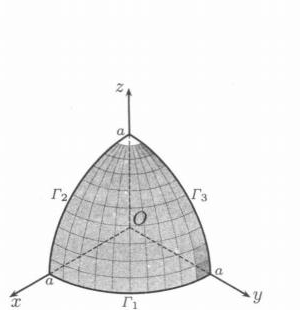
\includegraphics[width=.36\linewidth]{figures/lower/ch24/fig-24-1.png}
  \par 图 24.1
\end{center}

\subsection{练习题}

\begin{xexercise}[1]
计算下列第一型曲线积分：
\begin{enumerate}[label=(\arabic*)]
  \item $\displaystyle\int_C(x^{4/3}+y^{4/3})\,\dd s$，其中 $C$ 为星形线 $x^{2/3}+y^{2/3}=a^{2/3}$；
  \item $\displaystyle\int_C \ee^{\sqrt{x^2+y^2}}\,\dd s$，其中 $C$ 为由曲线 $r=a,\ \varphi=0,\ \varphi=\frac\pi4$（$r$ 和 $\varphi$ 为极坐标）所界的凸围线；
  \item $\displaystyle\int_C\abs{y}\,\dd s$，其中 $C$ 为双纽线 $(x^2+y^2)^2=a^2(x^2-y^2)$；
  \item $\displaystyle\int_C\frac{\dd s}{y^2}$，其中 $C$ 为悬链线 $y=a\operatorname{ch}\frac xa$；
  \item $\displaystyle\int_C z\,\dd s$，其中 $C$ 为曲线 $x^2+y^2=z^2,\ y^2=ax$ 从 $(0,0,0)$ 到 $(a,a,\sqrt2a)$ 的弧。
\end{enumerate}
\end{xexercise}
\begin{xsolution}
\begin{enumerate}[label=(\arabic*)]
\item 取星形线参数
\[
  x=a\cos^3 t,\qquad y=a\sin^3 t,\qquad 0\le t\le2\pi.
\]
则
\[
  \dd s=3a\abs{\sin t\cos t}\,\dd t,
\]
且
\[
  x^{4/3}+y^{4/3}=a^{4/3}(\cos^4t+\sin^4t).
\]
由四象限对称性，
\begin{align*}
  I
  &=12a^{7/3}\int_0^{\pi/2}(\cos^4t+\sin^4t)\sin t\cos t\,\dd t\\
  &=12a^{7/3}\left(\frac16+\frac16\right)
   =4a^{7/3}.
\end{align*}

\item $C$ 是扇形 $0\le r\le a,\ 0\le\varphi\le\pi/4$ 的边界。两条径向边上 $\dd s=\dd r$，圆弧上 $r=a$ 且 $\dd s=a\,\dd\varphi$，故
\begin{align*}
  I
  &=2\int_0^a\ee^r\,\dd r
    +\int_0^{\pi/4}\ee^a a\,\dd\varphi\\
  &=2(\ee^a-1)+\frac{\pi a}{4}\ee^a.
\end{align*}

\item 双纽线用极坐标表示为
\[
  r^2=a^2\cos2\theta.
\]
先算右叶，$-\pi/4\le\theta\le\pi/4$。有
\[
  r=a\sqrt{\cos2\theta},\qquad
  \dd s=\sqrt{r^2+(r')^2}\,\dd\theta
  =\frac{a}{\sqrt{\cos2\theta}}\,\dd\theta.
\]
因 $\abs y=r\abs{\sin\theta}$，故右叶上的积分为
\[
  a^2\int_{-\pi/4}^{\pi/4}\abs{\sin\theta}\,\dd\theta
  =a^2(2-\sqrt2).
\]
左右两叶相等，因此
\[
  I=2a^2(2-\sqrt2)=(4-2\sqrt2)a^2.
\]

\item 对整条悬链线 $y=a\operatorname{ch}(x/a)$，$-\infty<x<+\infty$，
\[
  \dd s=\operatorname{ch}(x/a)\,\dd x.
\]
于是
\[
  I=\frac1{a^2}\int_{-\infty}^{+\infty}\frac{\dd x}{\operatorname{ch}(x/a)}
  =\frac1a\int_{-\infty}^{+\infty}\frac{\dd u}{\operatorname{ch}u}
  =\frac\pi a.
\]

\item 由 $y^2=ax$，在所给弧上可令
\[
  y=at,\qquad x=at^2,\qquad
  z=at\sqrt{1+t^2},\qquad 0\le t\le1.
\]
于是
\[
  \dd s
  =a\sqrt{\frac{8t^4+9t^2+2}{1+t^2}}\,\dd t,
\]
从而
\[
  z\,\dd s=a^2t\sqrt{8t^4+9t^2+2}\,\dd t.
\]
令 $u=t^2$，得
\[
  I=\frac{a^2}{2}\int_0^1\sqrt{8u^2+9u+2}\,\dd u.
\]
又
\[
  8u^2+9u+2=\frac1{32}\bigl[(16u+9)^2-17\bigr],
\]
故直接积分得到
\[
  I=\frac{\sqrt2a^2}{512}
  \left[
    100\sqrt{38}-72
    -17\ln\frac{25+4\sqrt{38}}{17}
  \right].
\]
\end{enumerate}
\end{xsolution}
\begin{xexercise}[2]
求下列空间曲线的弧长：
\begin{enumerate}[label=(\arabic*)]
  \item $y=a\arcsin\frac xa,\ z=\frac a4\ln\frac{a-x}{a+x}$ 从 $(0,0,0)$ 到 $(x_0,y_0,z_0)$；
  \item $x^2+y^2+z^2=a^2,\ \sqrt{x^2+y^2}\operatorname{ch}\left(\arctan\frac yx\right)=a$ 从 $(a,0,0)$ 到 $(x,y,z)$。
\end{enumerate}
\end{xexercise}
\begin{xsolution}
\begin{enumerate}[label=(\arabic*)]
\item 以 $x$ 为参数。由题面中的反正弦和对数可知端点必须满足 $\abs{x_0}<a$。由
\[
  y=a\arcsin\frac xa,
  \qquad
  z=\frac a4\ln\frac{a-x}{a+x}
\]
得
\[
  \frac{\dd y}{\dd x}=\frac{a}{\sqrt{a^2-x^2}},
  \qquad
  \frac{\dd z}{\dd x}=-\frac{a^2}{2(a^2-x^2)}.
\]
于是
\begin{align*}
  \frac{\dd s}{\dd x}
  &=\sqrt{1+\frac{a^2}{a^2-x^2}
      +\frac{a^4}{4(a^2-x^2)^2}}\\
  &=1+\frac{a^2}{2(a^2-x^2)}.
\end{align*}
弧长微元应取非负值，因此
\begin{align*}
  L
  &=\abs{\int_0^{x_0}\left(1+\frac{a^2}{2(a^2-x^2)}\right)\,\dd x}\\
  &=\abs{x_0+\frac a4\ln\frac{a+x_0}{a-x_0}}
   =\abs{x_0-z_0}.
\end{align*}
又 $z_0$ 与 $x_0$ 异号，故也可写成
\[
  L=\abs{x_0}+\abs{z_0}.
\]

\item 令
\[
  \theta=\arctan\frac yx,
  \qquad \rho=\sqrt{x^2+y^2}.
\]
第二个方程给出
\[
  \rho=a\operatorname{sech}\theta.
\]
再由球面方程可在一条连通分支上写成
\[
  z=\pm a\tanh\theta.
\]
在柱坐标中
\[
  \dd s^2=\dd\rho^2+\rho^2\,\dd\theta^2+\dd z^2
  =2a^2\operatorname{sech}^2\theta\,\dd\theta^2.
\]
因此从 $(a,0,0)$ 到给定点的弧长为（此时 $\abs z<a$）
\[
  L=\sqrt2a\abs{\int_0^{\theta_0}\operatorname{sech}\theta\,\dd\theta}
  =\sqrt2a\arctan\frac{\abs z}{\sqrt{a^2-z^2}}
  =\sqrt2a\arcsin\frac{\abs z}{a}.
\]
\end{enumerate}
\end{xsolution}
\begin{xexercise}[3]
计算均匀的曲线 $y=a\operatorname{ch}\frac xa$ 从 $(0,a)$ 到 $(b,h)$ 的弧的质心坐标。
\end{xexercise}
\begin{xsolution}
令
\[
  \beta=\frac ba,
  \qquad h=a\operatorname{ch}\beta.
\]
曲线为 $y=a\operatorname{ch}(x/a)$，$0\le x\le b$，且
\[
  \dd s=\operatorname{ch}(x/a)\,\dd x.
\]
总长（亦即单位线密度下的质量）为
\[
  m=\int_0^b\dd s=a\operatorname{sh}\beta
   =\sqrt{h^2-a^2}.
\]
于是
\begin{align*}
  \bar x
  &=\frac1m\int_0^b x\operatorname{ch}(x/a)\,\dd x\\
  &=b-a\frac{\operatorname{ch}\beta-1}{\operatorname{sh}\beta}
   =b-\frac{a(h-a)}{\sqrt{h^2-a^2}},
\end{align*}
而
\begin{align*}
  \bar y
  &=\frac1m\int_0^b a\operatorname{ch}^2(x/a)\,\dd x\\
  &=\frac h2+\frac{ab}{2\sqrt{h^2-a^2}}.
\end{align*}
故质心为
\[
  \left(
  b-\frac{a(h-a)}{\sqrt{h^2-a^2}},
  \frac h2+\frac{ab}{2\sqrt{h^2-a^2}}
  \right).
\]
\end{xsolution}
\begin{xexercise}[4]
设 $\Gamma=\wideparen{AB}$ 是 $\RR^n$ 中的简单可求长曲线，$\Gamma$ 的弧长记为 $L$。对每一个 $s\in[0,L]$，存在惟一的 $\vect{x}\in\Gamma$，$\vect{x}=(x_1,x_2,\ldots,x_n)$，使得 $\Gamma$ 上从 $A$ 到 $\vect{x}$ 的曲线段 $\wideparen{A\vect{x}}$ 的弧长等于 $s$，由此定义了一个 $[0,L]$ 上的函数
\begin{equation}
  \vect{x}=\vect{x}(s),\qquad 0\le s\le L.
  \tag{24.4}
  \label{eq:24.4}
\end{equation}
即曲线 $\Gamma$ 以弧长 $s$ 为参数的参数方程为 (24.4)。设 $f$ 是定义在 $\Gamma$ 上的函数，如果 $f$ 在 $\Gamma$ 上的第一型曲线积分存在，则
\[
  \int_\Gamma f(\vect{x})\,\dd s=\int_0^L f\bigl(\vect{x}(s)\bigr)\,\dd s.
\]
\end{xexercise}
\begin{xsolution}
由弧长参数的定义，任取
\[
  0=s_0<s_1<\cdots<s_m=L,
\]
其在曲线上对应的点为
\[
  \vect{x}(s_0),\vect{x}(s_1),\ldots,\vect{x}(s_m).
\]
第 $i$ 段曲线的弧长恰为
\[
  \Delta s_i=s_i-s_{i-1}.
\]
反过来，$\Gamma$ 上任一保持次序的分割也唯一对应于 $[0,L]$ 的一个分割。若在第 $i$ 段选取
$\xi_i=\vect{x}(\sigma_i)$，$s_{i-1}\le\sigma_i\le s_i$，则第一型曲线积分定义中的和为
\[
  \sum_{i=1}^m f(\xi_i)\Delta s_i
  =\sum_{i=1}^m f(\vect{x}(\sigma_i))(s_i-s_{i-1}),
\]
这正是函数 $f(\vect{x}(s))$ 在 $[0,L]$ 上的 Riemann 和。两边取分割直径趋于零的极限，即得
\[
  \int_\Gamma f(\vect{x})\,\dd s
  =\int_0^L f(\vect{x}(s))\,\dd s.
\]
\end{xsolution}


\section{第二型曲线积分}

\subsection{第二型曲线积分的定义和计算}

第二型曲线积分的物理背景之一是质点受力沿曲线运动所做的功。因此我们给定了曲线的起点和终点。这样的曲线称为有向曲线。下面以 $\RR^3$ 为例定义第二型曲线积分。设 $\Gamma=\wideparen{AB}$ 是 $\RR^3$ 中一条简单可求长的有向曲线
\[
  \vect{F}=\vect{F}(x,y,z)=P(x,y,z)\vect{i}+Q(x,y,z)\vect{j}+R(x,y,z)\vect{k}
\]
为定义在 $\Gamma$ 上的向量值函数。对于与 $\Gamma$ 方向一致的任意分割 $T$，
\[
  T\colon A=A_0,A_1,A_2,\ldots,A_m=B,
\]
记 $A_i=(x_i,y_i,z_i)$，$\Delta x_i=x_i-x_{i-1}$，$\Delta y_i=y_i-y_{i-1}$，$\Delta z_i=z_i-z_{i-1}$，$\Delta S_i$ 为曲线段 $\wideparen{A_{i-1}A_i}$ 的弧长，$d(T)=\max_{1\le i\le m}\{\Delta S_i\}$。任取 $(\xi_i,\eta_i,\zeta_i)\in\wideparen{A_{i-1}A_i}$，如果极限
\[
  \lim_{d(T)\to0}\sum_{i=1}^m\bigl[P(\xi_i,\eta_i,\zeta_i)\Delta x_i+Q(\xi_i,\eta_i,\zeta_i)\Delta y_i+R(\xi_i,\eta_i,\zeta_i)\Delta z_i\bigr]
\]
存在且极限与 $\Gamma$ 的具体分法以及 $(\xi_i,\eta_i,\zeta_i)$ 的具体取法无关，则称 $\vect{F}$ 沿 $\Gamma$ 的第二型曲线积分存在，极限值称为 $\vect{F}$ 沿 $\Gamma$ 的第二型曲线积分，记为
\[
  I=\int_\Gamma P(x,y,z)\,\dd x+Q(x,y,z)\,\dd y+R(x,y,z)\,\dd z
\]
或
\[
  I=\int_\Gamma \vect{F}(x,y,z)\cdot\dd\vect{r}.
\]
第二型曲线积分又称为对坐标的积分。

若逐段光滑的有向曲线 $\Gamma$ 有参数表示
\[
  x=x(t),\qquad y=y(t),\qquad z=z(t),\qquad a\le t\le b,
\]
其中 $[a,b]$ 是实轴上的有向区间，参数 $t$ 从 $a$ 变到 $b$ 与 $\Gamma$ 的定向一致，设 $P(x,y,z)$、$Q(x,y,z)$、$R(x,y,z)$ 在 $\Gamma$ 上连续，则
\begin{align*}
  &\int_\Gamma P(x,y,z)\,\dd x+Q(x,y,z)\,\dd y+R(x,y,z)\,\dd z\\
  &\qquad=\int_a^b\bigl[P(x(t),y(t),z(t))x'(t)+Q(x(t),y(t),z(t))y'(t)+R(x(t),y(t),z(t))z'(t)\bigr]\,\dd t.
\end{align*}

\begin{xexample}[24.2.1]
计算积分
\[
  I=\int_C(x^2+2xy)\,\dd y,
\]
其中 $C$ 表示逆时针方向的上半椭圆 $\dfrac{x^2}{a^2}+\dfrac{y^2}{b^2}=1$。
\end{xexample}
\begin{xsolution}
利用椭圆的参数表达式
\[
  x=a\cos t,\qquad y=b\sin t,
\]
按给定方向 $t$ 由 $0$ 变到 $\pi$，将 $x,y$ 用 $t$ 的表达式代入并用 $b\cos t\,\dd t$ 来代替 $\dd y$，得
\begin{align*}
  I&=\int_0^\pi(a^2\cos^2t+2ab\cos t\sin t)b\cos t\,\dd t\\
   &=a^2b\int_0^\pi\cos^3t\,\dd t+2ab^2\int_0^\pi\cos^2t\sin t\,\dd t=\frac43ab^2.
\end{align*}
\end{xsolution}

\begin{xexample}[24.2.2]
求 $I=\displaystyle\int_\Gamma y^2\,\dd x+z^2\,\dd y+x^2\,\dd z$，其中 $\Gamma$ 为曲线
\[
  \begin{cases}
    x^2+y^2+z^2=a^2,\\
    x^2+y^2=ax\quad(a>0)
  \end{cases}
\]
上 $z\ge0$ 的部分（即 Viviani 体的顶部曲线），且从 $x$ 轴正向看 $\Gamma$ 是逆时针方向。
\end{xexample}
\begin{xsolution}
参见图 22.11。先求曲线 $\Gamma$ 的参数表达式。若以 $x,y,z$ 之一为参数，则要涉及开方运算，出现分支，很不方便。从第二个方程易见引入柱坐标
\[
  x=r\cos\theta,\qquad y=r\sin\theta,\qquad z=z,
\]
于是 $\Gamma$ 的参数方程为
\[
  x=a\cos^2\theta,\qquad y=a\cos\theta\sin\theta,
\]
\[
  z=\sqrt{a^2-r^2}=a\abs{\sin\theta},\qquad -\frac\pi2\le\theta\le\frac\pi2.
\]
根据曲线定向，有
\[
  I=\int_{-\pi/2}^{\pi/2}\left[a^2\cos^2\theta\sin^2\theta\cdot2a\cos\theta(-\sin\theta)+a^2\sin^2\theta\cdot a(\cos^2\theta-\sin^2\theta)+a^2\cos^4\theta\cdot z'(\theta)\right]\,\dd\theta.
\]
第一项是奇函数，且因子 $z(\theta)$ 是偶函数，所以 $z'(\theta)$ 是奇函数，故第三项也是奇函数，于是
\[
  I=\int_{-\pi/2}^{\pi/2}a^3\sin^2\theta(\cos^2\theta-\sin^2\theta)\,\dd\theta
  =2a^3\int_0^{\pi/2}(\sin^2\theta-2\sin^4\theta)\,\dd\theta=-\frac\pi4a^3.
\]
\end{xsolution}

有的时候空间曲线的参数方程不容易写出或写出来比较复杂，我们可以借助下列命题把问题转化为平面曲线的曲线积分。

\begin{xproposition}[24.2.1]
设逐段光滑曲线 $\Gamma$ 在光滑曲面 $z=f(x,y)$ 上，曲线 $\Gamma$ 在 $xOy$ 平面上的投影曲线为 $\gamma$，函数 $P(x,y,z)$ 在 $\Gamma$ 上连续，则
\[
  \oint_\Gamma P(x,y,z)\,\dd x=\oint_\gamma P(x,y,f(x,y))\,\dd x,
\]
其中 $\gamma$ 的定向与 $\Gamma$ 的定向一致。
\end{xproposition}
\begin{xproof}
设 $\gamma$ 的参数方程为
\[
  x=\varphi(t),\qquad y=\psi(t),\qquad a\le t\le b,
\]
则空间曲线 $\Gamma$ 的方程为
\[
  x=\varphi(t),\qquad y=\psi(t),\qquad z=f(\varphi(t),\psi(t)).
\]
于是
\[
  \oint_\Gamma P(x,y,z)\,\dd x=\int_a^bP[\varphi(t),\psi(t),f(\varphi(t),\psi(t))]\varphi'(t)\,\dd t
  =\oint_\gamma P(x,y,f(x,y))\,\dd x.
\]
\end{xproof}

\subsection{两类曲线积分的关系}

坐标微元 $\dd\vect{r}=\vect{\tau}\,\dd s$，其中 $\vect{\tau}$ 为曲线沿指定方向的单位切向，因而就有
\[
  \int_\Gamma \vect{F}(\vect{x})\cdot\dd\vect{r}=\int_\Gamma(\vect{F}(\vect{x})\cdot\vect{\tau})\,\dd s.
\]
对于空间曲线 $\Gamma$，设 $\cos\alpha,\cos\beta,\cos\gamma$ 是切方向余弦，则
\begin{equation}
  \int_\Gamma P\,\dd x+Q\,\dd y+R\,\dd z=\int_\Gamma(P\cos\alpha+Q\cos\beta+R\cos\gamma)\,\dd s.
  \tag{24.5}
  \label{eq:24.5}
\end{equation}
当 $\Gamma$ 为平面曲线时，取法线的方向 $\vect{n}$ 与切线的方向 $\vect{\tau}$ 的夹角 $\angle(\vect{n},\vect{\tau})=\frac\pi2$，见图 24.2，则
\[
  \angle(x,\vect{n})=\angle(x,\vect{\tau})+\angle(\vect{\tau},\vect{n})=\alpha-\frac\pi2,
\]
即
\[
  \cos\alpha=-\sin(x,\vect{n}),\qquad \sin\alpha=\cos(x,\vect{n}).
\]
于是 $\Gamma$ 为平面曲线时
\begin{equation}
  \int_\Gamma P\,\dd x+Q\,\dd y=\int_\Gamma[-P\sin(x,\vect{n})+Q\cos(x,\vect{n})]\,\dd s.
  \tag{24.6}
  \label{eq:24.6}
\end{equation}

\begin{center}
  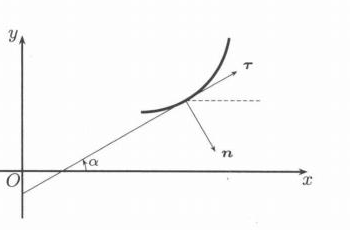
\includegraphics[width=.38\linewidth]{figures/lower/ch24/fig-24-2.png}
  \par 图 24.2
\end{center}

\subsection{第二型曲线积分的应用}

\textbf{求变力做功}

\begin{xexample}[24.2.3]
已知一平面力场，它的方向指向坐标原点，它的大小与它到原点的距离 $r$ 的平方成反比：
\[
  F=\frac{\mu}{r^2},
\]
其中 $\mu$ 为常数。计算当质量 $m=1$ 的质点自位置 $A$ 移动到位置 $B$（不通过原点）时力场做的功。
\end{xexample}
\begin{xsolution}
以 $(x,y)$ 表示点的坐标。设力与 $x$ 轴的夹角 $\theta$，则
\[
  \cos\theta=-\frac xr,\qquad \sin\theta=-\frac yr.
\]
于是力在 $x,y$ 方向的分量分别为
\[
  F_1(x,y)=F\cos\theta=-\mu\frac{x}{r^3},\qquad
  F_2(x,y)=F\sin\theta=-\mu\frac{y}{r^3}.
\]
而功可表示为曲线积分
\[
  w=-\mu\int_{\wideparen{AB}}\frac{x\,\dd x+y\,\dd y}{r^3}.
\]
容易看出
\begin{equation}
  -\frac{x\,\dd x+y\,\dd y}{r^3}=\dd\frac1r.
  \tag{24.7}
  \label{eq:24.7}
\end{equation}
且如将 $x,y$ 用参数表达式 $x=\varphi(t),\ y=\psi(t)$ 代入，其中 $a\le t\le b$，并令
\[
  r=\sqrt{x^2+y^2}=\sqrt{\varphi^2(t)+\psi^2(t)}
\]
时，等式 (24.7) 仍成立。于是
\[
  w=\mu\int_a^b\dd\frac1r=\mu\left.\frac1r\right|_a^b
  =\mu\left(\frac1{r_B}-\frac1{r_A}\right),
\]
其中 $r_A,r_B$ 分别表示原点到点 $A,B$ 的距离。
\end{xsolution}

\textbf{梯度曲线}\quad 设 $f$ 是区域 $D\subset\RR^3$ 上的 $C^1$ 函数，并设 $\nabla f$ 是在 $D$ 上处处不为零的向量。若 $\Gamma$ 是自某点 $(x_0,y_0,z_0)\in D$ 出发的可微曲线，它的每一点的切线方向与 $f$ 的梯度方向一致，就称 $\Gamma$ 为 $f$ 在 $D$ 上的梯度曲线。设 $\Gamma$ 的参数方程为
\[
  x=x(t),\qquad y=y(t),\qquad z=z(t),
\]
则可取 $x(t),y(t)$ 和 $z(t)$ 满足如下微分方程组：
\begin{equation}
  \frac{\dd x}{\dd t}=\frac1{\abs{\nabla f}}\frac{\partial f}{\partial x},\qquad
  \frac{\dd y}{\dd t}=\frac1{\abs{\nabla f}}\frac{\partial f}{\partial y},\qquad
  \frac{\dd z}{\dd t}=\frac1{\abs{\nabla f}}\frac{\partial f}{\partial z}.
  \tag{24.8}
  \label{eq:24.8}
\end{equation}
初始值为 $x(0)=x_0,\ y(0)=y_0,\ z(0)=z_0$。由常微分方程组解的存在性定理和延拓定理\footnote{可参考任何一本常微分方程的教科书，我们所用的知识并没有超出大学二年级的范围。这些材料均可作为曲线积分复习时的补充。}，$x(t),y(t)$ 和 $z(t)$ 在 $D$ 内存在并可延伸到 $D$ 的边界。由 (24.8)，$\Gamma$ 的弧长微分满足
\[
  \dd s=\sqrt{[x'(t)]^2+[y'(t)]^2+[z'(t)]^2}\,\dd t=\dd t.
\]
下面我们借助 $\RR^2$ 中的梯度曲线重新讨论例题 21.3.3。这是著名的美国大学 Putnam 竞赛第二十八届的 B6 题，它公布的标准答案就是例题 21.3.3 的解答。我们现在可以将那里的梯度模的最小值的上界估计从 16 改进为 4。

\begin{xexample}[24.2.4]
设 $f(x,y)$ 在单位圆盘 $D=\{(x,y)\mid x^2+y^2\le1\}$ 上具有连续的一阶偏导数，且满足 $\abs{f(x,y)}\le1,\ \forall(x,y)\in D$。证明：存在点 $p_0(x_0,y_0)\in\operatorname{int}D=\{(x,y)\mid x^2+y^2<1\}$，使得
\[
  (f_x^2+f_y^2)|_{(x_0,y_0)}\le4.
\]
\end{xexample}
\begin{xproof}
如果有点 $(x_0,y_0)$，使 $\nabla f(x_0,y_0)=0$，即 $f_x(x_0,y_0)=f_y(x_0,y_0)=0$，则估计式成立。如果 $\nabla f$ 在 $D$ 中处处不为零向量，则 $f$ 在 $D$ 中的梯度曲线存在。设 $\Gamma$ 是 $f$ 在 $D$ 中的梯度曲线，其参数方程为
\[
  x=x(t),\qquad y=y(t),\qquad t\in[0,T],
\]
$\Gamma$ 的起点为原点，终点为 $(x(T),y(T))$。由曲线积分公式得到
\begin{align*}
  f(x(T),y(T))-f(0,0)
  &=\int_0^T\left(\frac{\partial f}{\partial x}x'(t)+\frac{\partial f}{\partial y}y'(t)\right)\,\dd t\\
  &=\int_0^T\frac{\dfrac{\partial f}{\partial x}x'(t)+\dfrac{\partial f}{\partial y}y'(t)}{\sqrt{[x'(t)]^2+[y'(t)]^2}}\sqrt{[x'(t)]^2+[y'(t)]^2}\,\dd t\\
  &=\int_\Gamma(\nabla f(x,y)\cdot\vect{\tau})\,\dd s.
\end{align*}
设 $l$ 是 $\Gamma$ 的弧长，并且 $\Gamma$ 自原点出发到达 $D$ 的边界，则 $l\ge1$。如果在 $\operatorname{int}D$ 上处处有 $\nabla f(x,y)\cdot\vect{\tau}>2$，则就有
\[
  2\ge\abs{f(x(T),y(T))-f(0,0)}>2l\ge2,
\]
引出矛盾。因此存在 $(x_0,y_0)\in\operatorname{int}D$，使 $\nabla f(x_0,y_0)\cdot\vect{\tau}\le2$。又因为 $\nabla f$ 与 $\vect{\tau}$ 相切，故 $\nabla f(x_0,y_0)\cdot\vect{\tau}=\abs{\nabla f(x_0,y_0)}\le2$，即 $(f_x^2+f_y^2)|_{(x_0,y_0)}\le4$。
\end{xproof}

\begin{xremark}
用梯度曲线来估计函数差的下界也是十分有效的，其依据就是函数沿梯度方向增长最快。用这样的方法可以证明如下的\textbf{高维中值定理}（见《美国数学月刊》(1999) 第 106 卷 674--675 页，其证明作为第二组参考题 2）。

设 $f(\vect{x})$ 为定义在以 $r$ 为半径的 $n$ 维球
\[
  D=\{\vect{x}=(x_1,x_2,\ldots,x_n)\mid x_1^2+x_2^2+\cdots+x_n^2\le r^2\}
\]
上的连续可微函数，则存在点 $p_0=(p_1^0,p_2^0,\ldots,p_n^0)\in\operatorname{int}D$，使
\[
  \max_{\vect{x}\in D}\{f(\vect{x})\}-\min_{\vect{x}\in D}\{f(\vect{x})\}=\abs{\nabla f(p_0)}\cdot2r.
\]
利用这个结果或修改上述例题中的证明可以将估计值 4 改进为最佳的估计值 1。
\end{xremark}

\subsection{练习题}

\begin{xexercise}[1]
计算 $\displaystyle\int_Lxy\,\dd x+(y-x)\,\dd y$，其中 $L$ 为曲线，$\wideparen{AB}$ 方向为由 $A$ 到 $B$，$A=(1,1),\ B=(2,3)$：
\begin{enumerate}[label=(\arabic*)]
  \item $\wideparen{AB}$ 是直线 $AB$；
  \item $\wideparen{AB}$ 的方程是 $y=2(x-1)^2+1$；
  \item $\wideparen{AB}$ 是折线 $ADB$，$D=(2,1)$。
\end{enumerate}
\end{xexercise}
\begin{xsolution}
记
\[
  \omega=xy\,\dd x+(y-x)\,\dd y.
\]
\begin{enumerate}[label=(\arabic*)]
\item 直线段 $AB$ 取
\[
  x=1+t,\qquad y=1+2t,\qquad0\le t\le1.
\]
则
\[
  \omega=(1+5t+2t^2)\,\dd t,
\]
故
\[
  \int_{AB}\omega=\int_0^1(1+5t+2t^2)\,\dd t=\frac{25}{6}.
\]

\item 令 $u=x-1$，则 $0\le u\le1$，$x=u+1$，$y=2u^2+1$，$\dd y=4u\,\dd u$。于是
\[
  \omega=(10u^3-2u^2+u+1)\,\dd u,
\]
从而
\[
  \int_{\wideparen{AB}}\omega=\frac{10}{4}-\frac23+\frac12+1=\frac{10}{3}.
\]

\item 在 $A\to D$ 上 $y=1$，故
\[
  \int_{AD}\omega=\int_1^2x\,\dd x=\frac32.
\]
在 $D\to B$ 上 $x=2$，故
\[
  \int_{DB}\omega=\int_1^3(y-2)\,\dd y=0.
\]
因此
\[
  \int_{ADB}\omega=\frac32.
\]
\end{enumerate}
\end{xsolution}
\begin{xexercise}[2]
求 $\displaystyle\int_C\frac{x}{y}\,\dd x+\frac1{y-a}\,\dd y$，其中 $C$ 是旋轮线 $x=a(t-\sin t),\ y=a(1-\cos t)$ 对应于 $t=\frac\pi6$ 到 $t=\frac\pi3$ 的一段。
\end{xexercise}
\begin{xsolution}
由
\[
  x=a(t-\sin t),\quad y=a(1-\cos t),
\]
有
\[
  \dd x=a(1-\cos t)\,\dd t=y\,\dd t,
  \qquad
  \dd y=a\sin t\,\dd t,
\]
且 $y-a=-a\cos t$。故
\begin{align*}
  I
  &=\int_{\pi/6}^{\pi/3}
  \left[a(t-\sin t)-\tan t\right]\,\dd t\\
  &=a\left[\frac{t^2}{2}+\cos t\right]_{\pi/6}^{\pi/3}
    +\left[\ln\abs{\cos t}\right]_{\pi/6}^{\pi/3}\\
  &=a\left(\frac{\pi^2}{24}+\frac{1-\sqrt3}{2}\right)
    -\frac12\ln3.
\end{align*}
\end{xsolution}
\begin{xexercise}[3]
求 $\displaystyle\int_C(x+y)^2\,\dd x+(x^2-y^2)\,\dd y$，其中 $C$ 是以 $A(1,1),B(3,2),D(3,1)$ 为顶点的三角形，取顺时针方向。
\end{xexercise}
\begin{xsolution}
令
\[
  P=(x+y)^2,\qquad Q=x^2-y^2.
\]
则
\[
  \frac{\partial Q}{\partial x}-\frac{\partial P}{\partial y}
  =-2y.
\]
给定方向为顺时针，故由 Green 公式要取负号：
\[
  I=-\iint_D(-2y)\,\dd x\,\dd y
   =2\iint_Dy\,\dd x\,\dd y.
\]
三角形 $ABD$ 的面积为 $1$，其形心的 $y$ 坐标为
\[
  \frac{1+2+1}{3}=\frac43.
\]
因此
\[
  I=2\cdot1\cdot\frac43=\frac83.
\]
\end{xsolution}
\begin{xexercise}[4]
求 $\displaystyle\int_C4xy^2\,\dd x-3x^4\,\dd y$，其中 $C$ 是抛物线 $y=\frac12x^2$ 自 $(0,0)$ 到 $(2,2)$ 的一段。
\end{xexercise}
\begin{xsolution}
取 $x$ 为参数，$0\le x\le2$，$y=x^2/2$，$\dd y=x\,\dd x$。于是
\[
  4xy^2\,\dd x-3x^4\,\dd y
  =x^5\,\dd x-3x^5\,\dd x=-2x^5\,\dd x.
\]
故
\[
  I=-2\int_0^2x^5\,\dd x=-\frac{64}{3}.
\]
\end{xsolution}
\begin{xexercise}[5]
求 $\displaystyle\oint_C(y^2+z^2)\,\dd x+(z^2+x^2)\,\dd y+(x^2+y^2)\,\dd z$，其中 $C$ 是曲面 $x^2+y^2+z^2=2Rx,\ x^2+y^2=2ax$ 的交线（$0<a<R,z>0$），且由 $z$ 轴正向看是逆时针方向。
\end{xexercise}
\begin{xsolution}
记
\[
  S=x^2+y^2+z^2.
\]
原微分形式可写成
\[
  (S-x^2)\,\dd x+(S-y^2)\,\dd y+(S-z^2)\,\dd z
  =S\,\dd(x+y+z)-\frac13\dd(x^3+y^3+z^3).
\]
闭路上后一项积分为零；又在球面上 $S=2Rx$，故
\[
  I=2R\oint_Cx(\dd x+\dd y+\dd z)
   =2R\left(\oint_Cx\,\dd y+\oint_Cx\,\dd z\right).
\]
由两曲面方程相减得
\[
  z^2=2(R-a)x,
\]
所以 $x\,\dd z=\dfrac{z^2}{2(R-a)}\,\dd z$ 是全微分，闭路积分为零。曲线在 $xOy$ 平面上的投影为
\[
  x^2+y^2=2ax,
\]
即圆心 $(a,0)$、半径 $a$ 的圆。题设从 $z$ 轴正向看为逆时针，故投影取正向，
\[
  \oint_Cx\,\dd y=\pi a^2.
\]
因此
\[
  I=2\pi Ra^2.
\]
\end{xsolution}
\begin{xexercise}[6]
求 $\displaystyle\int_C y\,\dd x+z\,\dd y+x\,\dd z$，其中 $C$ 为球面上的曲线：
\[
  x=R\sin\varphi\cos\theta,\qquad y=R\sin\varphi\sin\theta,\qquad z=R\cos\varphi,
\]
\[
  R>0,\quad0\le\varphi\le\pi,\quad0\le\theta<2\pi,
\]
并且使 (1) $R,\varphi$ 为常数；或 (2) $R,\theta$ 为常数。
\end{xexercise}
\begin{xsolution}
\begin{enumerate}[label=(\arabic*)]
\item $R,\varphi$ 固定，令 $\theta$ 从 $0$ 增至 $2\pi$。记
\[
  A=R\sin\varphi,\qquad B=R\cos\varphi,
\]
则 $x=A\cos\theta,y=A\sin\theta,z=B$。于是
\[
  I=\int_0^{2\pi}\left[-A^2\sin^2\theta+AB\cos\theta\right]\,\dd\theta
  =-\pi R^2\sin^2\varphi.
\]

\item $R,\theta$ 固定，令 $\varphi$ 从 $0$ 增至 $\pi$。代入
\[
  x=R\sin\varphi\cos\theta,
  \quad y=R\sin\varphi\sin\theta,
  \quad z=R\cos\varphi
\]
后，含 $\sin\varphi\cos\varphi$ 的项积分为零，故
\[
  I=\frac{\pi R^2}{2}(\sin\theta-\cos\theta).
\]
若曲线取相反方向，上述结果相应变号。
\end{enumerate}
\end{xsolution}
\begin{xexercise}[7]
求 $\displaystyle\int_C(x^2+5y+3yz)\,\dd x+(5x+3xy-2)\,\dd y+(3xy-4z)\,\dd z$，其中 $C$ 为
\begin{enumerate}[label=(\arabic*)]
  \item $x=a\cos t,y=a\sin t,z=\dfrac{bt}{2\pi}$ 自 $t=0$ 到 $2\pi$ 的一段；
  \item 直线段 $AB$，起点 $A=(a,0,0)$，终点 $B=(a,0,b)$。
\end{enumerate}
\end{xexercise}
\begin{xsolution}
令
\[
  \omega=(x^2+5y+3yz)\,\dd x+(5x+3xy-2)\,\dd y+(3xy-4z)\,\dd z.
\]
可分解为
\[
  \omega=\dd\left(\frac{x^3}{3}+5xy-2y-2z^2+3xyz\right)
  +3x(y-z)\,\dd y.
\]
\begin{enumerate}[label=(\arabic*)]
\item 对螺旋线
\[
  x=a\cos t,\quad y=a\sin t,\quad z=\frac{bt}{2\pi},\quad0\le t\le2\pi,
\]
全微分部分从 $A$ 到 $B$ 的增量为 $-2b^2$。余项为
\begin{align*}
  3\int_Cx(y-z)\,\dd y
  &=3\int_0^{2\pi}a\cos t
    \left(a\sin t-\frac{bt}{2\pi}\right)a\cos t\,\dd t\\
  &=-\frac{3a^2b}{2\pi}\int_0^{2\pi}t\cos^2t\,\dd t
   =-\frac{3\pi a^2b}{2}.
\end{align*}
故
\[
  I=-\frac{3\pi a^2b}{2}-2b^2.
\]

\item 在线段 $AB$ 上 $x=a,y=0$，只有 $z$ 从 $0$ 到 $b$ 变化，故
\[
  I=\int_0^b(-4z)\,\dd z=-2b^2.
\]
\end{enumerate}
\end{xsolution}
\begin{xexercise}[8]
已知力场 $\vect{F}(x,y,z)=y\vect{i}-x\vect{j}+(x+y+z)\vect{k}$，求质点沿曲线 $x=a\cos t,\ y=a\sin t,\ z=\dfrac{bt}{2\pi}$ 从点 $A(a,0,0)$ 运动到点 $B(a,0,b)$ 时，力场 $\vect{F}$ 对质点所做的功。
\end{xexercise}
\begin{xsolution}
沿给定曲线
\[
  x=a\cos t,\quad y=a\sin t,\quad z=\frac{bt}{2\pi},\quad0\le t\le2\pi.
\]
功为
\[
  W=\int_Cy\,\dd x-x\,\dd y+(x+y+z)\,\dd z.
\]
前两项给出
\[
  \int_0^{2\pi}-a^2\,\dd t=-2\pi a^2.
\]
又 $\dd z=\dfrac{b}{2\pi}\,\dd t$，而 $x,y$ 的一周期积分均为零，故
\[
  \int_C(x+y+z)\,\dd z
  =\frac{b^2}{4\pi^2}\int_0^{2\pi}t\,\dd t
  =\frac{b^2}{2}.
\]
因此
\[
  W=-2\pi a^2+\frac{b^2}{2}.
\]
\end{xsolution}
\begin{xexercise}[9]
质点在力场 $\vect{F}=\dfrac{\ee^x}{1+y^2}\vect{i}+\dfrac{2y(1-\ee^x)}{(1+y^2)^2}\vect{j}$ 作用下，沿 $x^2+(y-1)^2=1$ 由点 $(0,0)$ 沿顺时针方向运动到点 $(1,1)$，求力场所做的功。
\end{xexercise}
\begin{xsolution}
记
\[
  P=\frac{\ee^x}{1+y^2},
  \qquad
  Q=\frac{2y(1-\ee^x)}{(1+y^2)^2}.
\]
有
\[
  \frac{\partial P}{\partial y}
  =\frac{\partial Q}{\partial x}
  =-\frac{2y\ee^x}{(1+y^2)^2},
\]
故在整个平面上为恰当微分。由 $\varphi_x=P$，可取
\[
  \varphi(x,y)=\frac{\ee^x-1}{1+y^2}.
\]
于是积分只与端点有关，
\[
  W=\varphi(1,1)-\varphi(0,0)
   =\frac{\ee-1}{2}.
\]
\end{xsolution}


\section{Green 公式}

\subsection{Green 公式}

Green 公式是将平面内的某区域上的二重积分与该区域边界上的一个特定的第二型曲线积分之间建立联系的一个重要公式。

设 $D$ 是 $\RR^2$ 内的一个有界闭区域，其边界 $\partial D$ 由光滑曲线或逐段光滑曲线组成。又设函数 $P,Q$ 在 $D$ 上有关于自变量 $x$ 和 $y$ 的连续偏导数，则下列 Green 公式成立：
\begin{equation}
  \iint_D\left(-\frac{\partial P}{\partial y}+\frac{\partial Q}{\partial x}\right)\,\dd x\,\dd y
  =\oint_{\partial D}P\,\dd x+Q\,\dd y,
  \tag{24.9}
  \label{eq:24.9}
\end{equation}
其中 $\partial D$ 的方向关于 $D$ 是正向的。

由平面上两类曲线积分之间的关系式 (24.6) 知，Green 公式 (24.9) 又可以写为
\begin{align*}
  \iint_D\left(\frac{\partial P}{\partial x}+\frac{\partial Q}{\partial y}\right)\,\dd x\,\dd y
  &=\oint_{\partial D}-Q\,\dd x+P\,\dd y\\
  &=\oint_{\partial D}[Q\sin(x,\vect{n})+P\cos(x,\vect{n})]\,\dd s,
\end{align*}
其中 $\vect{n}$ 是 $\partial D$ 上的单位外法向量。利用 $\angle(x,\vect{n})=\angle(x,y)+\angle(y,\vect{n})=\frac\pi2+\angle(y,\vect{n})$（参见图 24.2），则
\begin{equation}
  \iint_D\left(\frac{\partial P}{\partial x}+\frac{\partial Q}{\partial y}\right)\,\dd x\,\dd y
  =\oint_{\partial D}[P\cos(x,\vect{n})+Q\cos(y,\vect{n})]\,\dd s.
  \tag{24.10}
  \label{eq:24.10}
\end{equation}

公式 (24.9)，(24.10) 给我们提供了间接求平面上曲线积分的方法，即利用 Green 公式将曲线积分化为二重积分，即使曲线 $C$ 不封闭，也可以采用添加“辅助线”的方法去做。

\begin{xexample}[24.3.1]
$C$ 为抛物线 $2x=\pi y^2$ 自 $(0,0)$ 到 $(\frac\pi2,1)$ 的弧段，求
\[
  I=\int_C(2xy^3-y^2\cos x)\,\dd x+(1-2y\sin x+3x^2y^2)\,\dd y.
\]
\end{xexample}
\begin{xsolution}
令 $P(x,y)=2xy^3-y^2\cos x,\ Q(x,y)=1-2y\sin x+3x^2y^2$，则
\[
  -\frac{\partial P}{\partial y}+\frac{\partial Q}{\partial x}=0.
\]
为了利用 Green 公式 (24.9)，添加辅助线（如图 24.3），则
\[
  I=\int_C+\int_{\wideparen{BA}}+\int_{\wideparen{AO}}+\int_{\wideparen{AB}}+\int_{\wideparen{OA}}.
\]
由 Green 公式，前三项的积分为零，于是
\[
  I=\int_{\wideparen{AB}}+\int_{\wideparen{OA}}
  =\int_0^1\left[1-2y\sin\frac\pi2+3\left(\frac\pi2\right)^2y^2\right]\,\dd y
  =\frac{\pi^2}{4}.
\]
\end{xsolution}

\begin{center}
  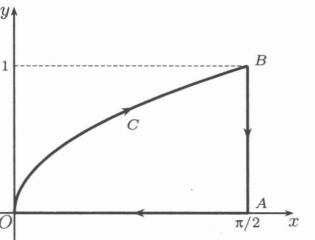
\includegraphics[width=.42\linewidth]{figures/lower/ch24/fig-24-3.png}
  \par 图 24.3
\end{center}

\begin{xexample}[24.3.2]
计算积分
\[
  I=\oint_C\frac{\cos(\vect{r},\vect{n})}{r}\,\dd s,
\]
其中 $C$ 为逐段光滑的简单闭曲线，$\vect{r}=(x,y),\ r=\abs{\vect{r}}=\sqrt{x^2+y^2},\ \vect{n}$ 是 $C$ 上的单位外法向量。
\end{xexample}
\begin{xsolution}
由 $\cos(\vect{r},\vect{n})=\dfrac{\vect{r}\cdot\vect{n}}r=\dfrac1r(x\cos(\vect{n},x)+y\cos(\vect{n},y))$ 得到
\[
  I=\oint_C\left(\frac{x}{r^2}\cos(\vect{n},x)+\frac{y}{r^2}\cos(\vect{n},y)\right)\,\dd s.
\]
当 $(0,0)$ 在 $C$ 外时，利用 Green 公式 (24.10)，则
\[
  I=\iint_D\left[\partial_x\left(\frac{x}{r^2}\right)+\partial_y\left(\frac{y}{r^2}\right)\right]\,\dd x\,\dd y=0,
\]
其中 $D$ 是以 $C$ 为边界的区域。

当 $(0,0)$ 在 $C$ 内时，以 $(0,0)$ 为圆心，以充分小的 $\varepsilon$ 为半径作圆 $C_\varepsilon$，使得 $C_\varepsilon$ 在 $C$ 内，以 $C$ 及 $C_\varepsilon$ 为边界的区域为 $D_\varepsilon$，则
\begin{align*}
  I={}&\oint_C\left(\frac{x}{r^2}\cos(\vect{n},x)+\frac{y}{r^2}\cos(\vect{n},y)\right)\,\dd s
  +\oint_{C_\varepsilon}\left(\frac{x}{r^2}\cos(\vect{n},x)+\frac{y}{r^2}\cos(\vect{n},y)\right)\,\dd s\\
  &-\oint_{C_\varepsilon}\left(\frac{x}{r^2}\cos(\vect{n},x)+\frac{y}{r^2}\cos(\vect{n},y)\right)\,\dd s.
\end{align*}
其中 $C_\varepsilon$ 上的单位法向量 $\vect{n}$ 的方向指向坐标原点。对前两项用 Green 公式，则
\[
  I=-\oint_{C_\varepsilon}\left(\frac{x}{r^2}\cos(\vect{n},x)+\frac{y}{r^2}\cos(\vect{n},y)\right)\,\dd s.
\]
在圆周 $C_\varepsilon$ 上，
\[
  \cos(\vect{n},x)=-\frac{x}{\varepsilon},\qquad
  \cos(\vect{n},y)=-\frac{y}{\varepsilon},\qquad r=\varepsilon,
\]
从而
\[
  I=\oint_{C_\varepsilon}\frac1\varepsilon\,\dd s=2\pi.
\]

当 $(0,0)\in C$ 时，过原点作曲线 $C$ 的切线 $OA,OB$，设 $OA,OB$ 的夹角为 $\theta$（见图 24.4），如果曲线 $C$ 在原点光滑，则 $\theta=\pi$。

作一个以 $(0,0)$ 点为心，$\varepsilon$ 为半径的圆 $B_\varepsilon$，记 $B_\varepsilon$ 的圆周在 $C$ 内的部分为 $C_\varepsilon$，由上面的计算知
\[
  I=\lim_{\varepsilon\to0}\int_{C_\varepsilon}\frac1\varepsilon\,\dd s
  =\lim_{\varepsilon\to0}\theta_\varepsilon=\theta,
\]
其中 $\theta_\varepsilon$ 是 $C_\varepsilon$ 所对应的圆心角。
\end{xsolution}

\begin{center}
  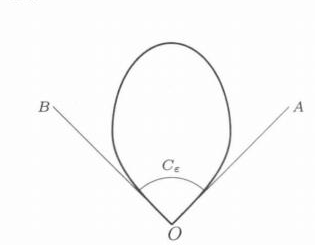
\includegraphics[width=.34\linewidth]{figures/lower/ch24/fig-24-4.png}
  \par 图 24.4
\end{center}

\begin{xremark}
注意使用 Green 公式的条件：$P,Q$ 在 $D$ 上连续可微。这正是在本题中要区分 $(0,0)$ 在 $C$ 外，$C$ 内和 $C$ 上三种情况讨论的缘故。许多学生没有能够注意到这里的区别，尤其是当点 $(0,0)$ 在 $C$ 内时，他们会错误地认为被积函数在 $C$ 上是连续可微的，因而 Green 公式就可以用了。
\end{xremark}

\begin{xexample}[24.3.3]
计算
\[
  I=\oint_C\frac{\ee^y}{x^2+y^2}\bigl[(x\sin x+y\cos x)\,\dd x+(y\sin x-x\cos x)\,\dd y\bigr],
\]
其中 $C\colon x^2+y^2=1$，取逆时针方向。
\end{xexample}
\begin{xsolution}
令
\[
  P(x,y)=\frac{\ee^y}{x^2+y^2}(x\sin x+y\cos x),
\]
\[
  Q(x,y)=\frac{\ee^y}{x^2+y^2}(y\sin x-x\cos x),
\]
由计算知 $\dfrac{\partial P}{\partial y}=\dfrac{\partial Q}{\partial x}$，从而可在不包含原点的区域上用 Green 公式。为此取 $C_\varepsilon\colon x^2+y^2=\varepsilon^2$，取逆时针方向，则
\[
  I=\oint_C-\oint_{C_\varepsilon}+\oint_{C_\varepsilon}.
\]
对等式右边前两项用 Green 公式，于是
\begin{align*}
  I&=\oint_{C_\varepsilon}\frac{\ee^y}{x^2+y^2}[(x\sin x+y\cos x)\,\dd x+(y\sin x-x\cos x)\,\dd y]\\
   &=\frac1{\varepsilon^2}\oint_{C_\varepsilon}\ee^y[(x\sin x+y\cos x)\,\dd x+(y\sin x-x\cos x)\,\dd y].
\end{align*}
记 $C_\varepsilon$ 围成的区域为 $D_\varepsilon$，再用一次 Green 公式，则
\[
  I=\frac1{\varepsilon^2}\iint_{D_\varepsilon}-2\ee^y\cos x\,\dd x\,\dd y.
\]
应用积分中值定理得到
\[
  I=\frac1{\varepsilon^2}(-2\pi\varepsilon^2\ee^\eta\cos\xi)
  =-2\pi\ee^\eta\cos\xi,
\]
其中 $(\xi,\eta)\in D_\varepsilon$。上述等式 $\forall\varepsilon>0$ 都对，令 $\varepsilon\to0$，得
\[
  I=\lim_{\varepsilon\to0+}(-2\pi\ee^\eta\cos\xi)=-2\pi.
\]
\end{xsolution}

\textbf{平面图形的面积}\quad 作为 Green 公式的直接推论，可以得到如下的面积公式。

由逐段光滑的简单曲线 $C$ 所界的面积 $S$ 可用曲线积分表示为
\[
  S=\oint_Cx\,\dd y=-\oint_Cy\,\dd x=\frac12\oint_Cx\,\dd y-y\,\dd x,
\]
其中曲线的正向为逆时针方向（参见上册 336--340 页的公式 (11.1) 及例题）。

\begin{xexample}[24.3.4]
计算双纽线
\begin{equation}
  (x^2+y^2)^2=a^2(x^2-y^2)
  \tag{24.11}
  \label{eq:24.11}
\end{equation}
所围区域的面积。
\end{xexample}
\begin{xsolution}
\textbf{解 1}\quad 由对称性只需计算第一、四象限的面积。令
\[
  x=r\cos\theta,\qquad y=r\sin\theta,\qquad -\frac\pi4\le\theta\le\frac\pi4,
\]
代入方程 (24.11) 得 $r=a\sqrt{\cos2\theta}$，则参数方程为
\[
  x(\theta)=a\cos\theta\sqrt{\cos2\theta},\qquad
  y(\theta)=a\sin\theta\sqrt{\cos2\theta},\qquad
  -\frac\pi4\le\theta\le\frac\pi4.
\]
并且
\[
  x'(\theta)=a(-\sin\theta)\sqrt{\cos2\theta}+a\cos\theta\frac{-\sin2\theta}{\sqrt{\cos2\theta}},
\]
\[
  y'(\theta)=a\cos\theta\sqrt{\cos2\theta}+a\sin\theta\frac{-\sin2\theta}{\sqrt{\cos2\theta}},
\]
所以
\[
  xy'-yx'=a^2\cos2\theta.
\]
由面积公式得到
\[
  S=2\cdot\frac12\oint x\,\dd y-y\,\dd x
  =\int_{-\pi/4}^{\pi/4}a^2\cos2\theta\,\dd\theta=a^2.
\]

\textbf{解 2（用定积分求面积）}\quad 在极坐标系中，双纽线 (24.11) 的方程为
\[
  r^2=a^2\cos2\theta,\qquad
  \theta\in\left[-\frac\pi4,\frac\pi4\right]\cup\left[\frac{3\pi}4,\frac{5\pi}4\right].
\]
于是
\[
  S=4\cdot\frac12\int_0^{\pi/4}r^2\,\dd\theta
  =2\int_0^{\pi/4}a^2\cos2\theta\,\dd\theta=a^2.
\]
\end{xsolution}

\subsection{平面曲线积分与路径无关的条件}

在力学上一种非常重要的力场是保守场。质点在保守场中移动，保守场所做的功只与质点的起点和终点的位置有关，与移动的具体路径无关。什么样的力场是保守场的问题从数学上看就是在什么条件下第二型曲线积分与路径无关，这个问题不仅具有明显的实际背景，而且在理论上也有很重要的意义。

设 $\Omega$ 是 $\RR^2$ 内的区域，$P(x,y),Q(x,y)$ 在 $\Omega$ 上连续，记
\[
  w=P(x,y)\,\dd x+Q(x,y)\,\dd y,
\]
任取点 $A,B\in\Omega$。$\Omega$ 内从 $A$ 到 $B$ 的一条逐段光滑的简单曲线称为 $\Omega$ 内从 $A$ 到 $B$ 的一条路径，对于 $\Omega$ 内从 $A$ 到 $B$ 的任意路径 $L$，如果第二型曲线积分
\[
  \int_Lw=\int_LP\,\dd x+Q\,\dd y
\]
只与 $A,B$ 有关，而与 $L$ 的具体选取无关，则称一阶微分形式 $w$ 在 $\Omega$ 内的\textbf{曲线积分与路径无关}。

如果平面区域 $D$ 内的任意简单闭曲线所包围的区域都完全在 $D$ 中，则称 $D$ 是\textbf{单连通区域}。设 $D$ 是平面内的单连通区域，$w=P\,\dd x+Q\,\dd y$，其中 $P,Q$ 都在 $D$ 上有连续的偏导数，则下列结论等价：
\begin{enumerate}[label=\arabic*.]
  \item 对 $D$ 内的任意一条闭曲线 $C$，有
  \[
    \oint_Cw=0;
  \]
  \item 对 $D$ 内的任一条路径 $C$，积分 $\int_Cw$ 仅与 $C$ 的起点和终点有关，而与所沿的路径无关；
  \item 在 $D$ 内（处处）成立
  \[
    \frac{\partial P}{\partial y}=\frac{\partial Q}{\partial x};
  \]
  \item 存在函数 $\varphi(x,y)$，使得在 $D$ 内成立
  \[
    \dd\varphi(x,y)=P(x,y)\,\dd x+Q(x,y)\,\dd y,
  \]
  即 $P\,\dd x+Q\,\dd y$ 是函数 $\varphi$ 的全微分。这时称 $\varphi$ 是 $w$ 的\textbf{势函数或原函数}，又称 $w$ 是一个\textbf{恰当微分形式}，此时
  \begin{equation}
    \varphi(x,y)=\int_{x_0}^xP(x,y_0)\,\dd x+\int_{y_0}^yQ(x,y)\,\dd y+C,
    \tag{24.12}
    \label{eq:24.12}
  \end{equation}
  其中 $(x_0,y_0)$ 为 $D$ 内任一点，$C$ 为任意常数，且
  \[
    \int_{(x_0,y_0)}^{(x,y)}P\,\dd x+Q\,\dd y
    =\left.\varphi\right|_{(x_0,y_0)}^{(x,y)}
    =\varphi(x,y)-\varphi(x_0,y_0).
  \]
\end{enumerate}

\begin{xremark}
回忆例题 24.2.3 的求解过程，由 (24.7) 知 $-\dfrac{x\,\dd x+y\,\dd y}{r^3}$ 是 $\dfrac1r$ 的全微分，则积分与路径无关，于是
\[
  w=\mu\left(\frac1{r_B}-\frac1{r_A}\right).
\]
但当时我们不知道可以这样计算第二型曲线积分。
\end{xremark}

\begin{xexample}[24.3.5]
设 $P(x,y),Q(x,y)$ 有连续偏导数，则 $\dfrac{\partial P}{\partial y}=\dfrac{\partial Q}{\partial x}$ 的充分必要条件是
\begin{equation}
  \int_{x_0}^xP(x,y)\,\dd x+\int_{y_0}^yQ(x_0,y)\,\dd y
  =\int_{x_0}^xP(x,y_0)\,\dd x+\int_{y_0}^yQ(x,y)\,\dd y.
  \tag{24.13}
  \label{eq:24.13}
\end{equation}
\end{xexample}
\begin{xproof}
先证充分性。设 (24.13) 成立，两边对 $x$ 求导，得
\[
  P(x,y)=P(x,y_0)+\int_{y_0}^y\frac{\partial Q}{\partial x}(x,y)\,\dd y.
\]
两边再对 $y$ 求导，则
\[
  \frac{\partial P}{\partial y}(x,y)=\frac{\partial Q}{\partial x}(x,y).
\]
再证必要性。由条件知 $w=P\,\dd x+Q\,\dd y$ 与积分路径无关。取路径为从 $(x_0,y_0)$ 经 $(x_0,y)$ 到 $(x,y)$，则势函数
\[
  \varphi(x,y)=\int_{x_0}^xP(x,y)\,\dd x+\int_{y_0}^yQ(x_0,y)\,\dd y+C_1.
\]
取路径为从 $(x_0,y_0)$ 经 $(x,y_0)$ 到 $(x,y)$，则
\[
  \varphi(x,y)=\int_{x_0}^xP(x,y_0)\,\dd x+\int_{y_0}^yQ(x,y)\,\dd y+C_2.
\]
令 $(x,y)=(x_0,y_0)$，得 $C_1=C_2$。
\end{xproof}

\begin{xexample}[24.3.6]
设 $a,b,c$ 为常数，满足 $ac-b^2>0$，
\[
  w=\frac{x\,\dd y-y\,\dd x}{ax^2+2bxy+cy^2},
\]
易见 $w$ 在 $(0,0)$ 以外的区域有定义，且为恰当微分形式。求 $w$ 关于原点 $(0,0)$ 的\textbf{循环常数} $\displaystyle\oint_Cw$，其中 $C$ 可取围绕 $(0,0)$ 的任一简单封闭曲线，并约定取逆时针方向为正向。
\end{xexample}
\begin{xsolution}
设
\[
  P(x,y)=\frac{-y}{ax^2+2bxy+cy^2},\qquad
  Q(x,y)=\frac{x}{ax^2+2bxy+cy^2},
\]
则 $\dfrac{\partial P}{\partial y}=\dfrac{\partial Q}{\partial x}$。可以看出，沿椭圆 $C$：
\[
  ax^2+2bxy+cy^2=1
\]
来计算曲线积分最为简便，因为此时
\[
  \oint_CP\,\dd x+Q\,\dd y=\oint_Cx\,\dd y-y\,\dd x,
\]
上述积分值恰为椭圆的面积的两倍，于是
\[
  \oint_Cw=\frac{2\pi}{\sqrt{ac-b^2}}.
\]
\end{xsolution}

\subsection{练习题}

\begin{xexercise}[1]
应用 Green 公式求下列第二型曲线积分：
\begin{enumerate}[label=(\arabic*)]
  \item $\displaystyle\oint_C(x^2+xy)\,\dd x+(x^2+y^2)\,\dd y$，$C$ 为由 $x=\pm1,y=\pm1$ 围成的正方形，取正向；
  \item 求 $\displaystyle\oint_C\ln\frac{2+y}{1+x^2}\,\dd x+\frac{x(y+1)}{2+y}\,\dd y$，$C$ 的定义同 (1)；
  \item 求 $\displaystyle\oint_C(x^2-y^2)\,\dd x-2xy\,\dd y$，$C$ 是由 $x^2+y^2=1,x=y$ 及 $y$ 轴围成的曲边三角形，取正向；
  \item 求 $\displaystyle\int_C\frac1{x^2+y^2}(x\,\dd y-y\,\dd x)$，其中 $C$ 是：(a) 旋轮线 $x=a(t-\sin t)-a\pi,\ y=a(1-\cos t)$ 对应于 $t=0$ 到 $t=2\pi$ 的一拱；(b) $(x-1)^2+(y-1)^2=1$ 从 $(2,1)$ 经上半圆到 $(0,1)$ 的一段弧。
\end{enumerate}
\end{xexercise}
\begin{xsolution}
\begin{enumerate}[label=(\arabic*)]
\item 令 $P=x^2+xy,Q=x^2+y^2$。则
\[
  Q_x-P_y=2x-x=x.
\]
区域是关于 $y$ 轴对称的正方形 $[-1,1]^2$，所以
\[
  \oint_C P\,\dd x+Q\,\dd y
  =\iint_{[-1,1]^2}x\,\dd x\,\dd y=0.
\]

\item 令
\[
  P=\ln\frac{2+y}{1+x^2},
  \qquad
  Q=\frac{x(y+1)}{2+y}.
\]
则
\[
  Q_x-P_y=\frac{y+1}{y+2}-\frac1{y+2}=\frac y{y+2}.
\]
故
\begin{align*}
  I
  &=\int_{-1}^1\int_{-1}^1\frac y{y+2}\,\dd x\,\dd y\\
  &=2\int_{-1}^1\left(1-\frac2{y+2}\right)\,\dd y
   =4-4\ln3.
\end{align*}

\item 令 $P=x^2-y^2,Q=-2xy$。有
\[
  Q_x-P_y=-2y-(-2y)=0.
\]
被积函数在整个平面上连续可微，所以无论该曲边三角形的具体形状如何，按闭曲线 Green 公式均有
\[
  I=0.
\]

\item 注意
\[
  \frac{x\,\dd y-y\,\dd x}{x^2+y^2}=\dd\arg(x+\ii y)
\]
在不经过原点的曲线上成立。
\begin{enumerate}[label=(\alph*)]
\item 旋轮线一拱经平移后从 $(-a\pi,0)$ 到 $(a\pi,0)$，且除端点外位于上半平面。沿给定参数方向，连续辐角从 $\pi$ 变到 $0$，故
\[
  I=-\pi.
\]
\item 圆弧从 $(2,1)$ 经上半圆到 $(0,1)$，全程位于第一、第二象限而不经过原点。故
\[
  I=\frac\pi2-\arctan\frac12=\arctan2.
\]
\end{enumerate}
\end{enumerate}
\end{xsolution}
\begin{xexercise}[2]
设 $f(x)$ 连续可微，$L$ 为逐段光滑闭曲线，证明：
\begin{enumerate}[label=(\arabic*)]
  \item $\displaystyle\oint_Lf(xy)(y\,\dd x+x\,\dd y)=0$；
  \item $\displaystyle\oint_Lf(x^2+y^2)(x\,\dd x+y\,\dd y)=0$。
\end{enumerate}
\end{xexercise}
\begin{xsolution}
\begin{enumerate}[label=(\arabic*)]
\item 取 $F$ 为 $f$ 的一个原函数，即 $F'=f$。由于
\[
  y\,\dd x+x\,\dd y=\dd(xy),
\]
所以
\[
  f(xy)(y\,\dd x+x\,\dd y)=\dd F(xy).
\]
闭曲线上的全微分积分为零，故所求积分为 $0$。

\item 取 $H$ 满足 $H'(u)=\frac12f(u)$。由于
\[
  x\,\dd x+y\,\dd y=\frac12\dd(x^2+y^2),
\]
有
\[
  f(x^2+y^2)(x\,\dd x+y\,\dd y)
  =\dd H(x^2+y^2).
\]
故闭路积分仍为 $0$。
\end{enumerate}
\end{xsolution}
\begin{xexercise}[3]
求 $\displaystyle\oint_C\frac{\partial u}{\partial n}\,\dd s$，其中 $u=x^2+y^2$，$C$ 为 $x^2+y^2=6x$，$n$ 为 $C$ 上的单位外法向量。
\end{xexercise}
\begin{xsolution}
$u=x^2+y^2$，故
\[
  \nabla u=(2x,2y),\qquad \Delta u=4.
\]
由 Green 公式的通量形式，
\[
  \oint_C\frac{\partial u}{\partial n}\,\dd s
  =\iint_D\Delta u\,\dd x\,\dd y.
\]
圆 $x^2+y^2=6x$ 的圆心为 $(3,0)$、半径为 $3$，面积为 $9\pi$，因此
\[
  \oint_C\frac{\partial u}{\partial n}\,\dd s
  =4\cdot9\pi=36\pi.
\]
\end{xsolution}
\begin{xexercise}[4]
设 $C$ 为逐段光滑的简单闭曲线，$l$ 为给定方向，证明：
\[
  \oint_C\cos(l,n)\,\dd s=0,
\]
其中 $n$ 为 $C$ 上的单位外法向量。
\end{xexercise}
\begin{xsolution}
设给定方向 $l$ 的单位向量为
\[
  \vect{e}=(\cos\alpha,\sin\alpha).
\]
则 $\cos(l,n)=\vect{e}\cdot\vect{n}$。常向量场 $\vect{e}$ 的散度为零，故由 Green 公式的通量形式
\[
  \oint_C\cos(l,n)\,\dd s
  =\oint_C\vect{e}\cdot\vect{n}\,\dd s
  =\iint_D\operatorname{div}\vect{e}\,\dd x\,\dd y=0.
\]
\end{xsolution}
\begin{xexercise}[5]
设 $C$ 为包围原点的逐段光滑的简单闭曲线，$a_{ij}\ (i,j=1,2)$ 均为常数，$X=a_{11}x+a_{12}y,\ Y=a_{21}x+a_{22}y$，$a_{11}a_{22}-a_{12}a_{21}\ne0$，证明：
\[
  \oint_C\frac{X\,\dd Y-Y\,\dd X}{X^2+Y^2}=2\pi\operatorname{sgn}(a_{11}a_{22}-a_{12}a_{21}).
\]
\end{xexercise}
\begin{xsolution}
记
\[
  A=\begin{pmatrix}a_{11}&a_{12}\\a_{21}&a_{22}\end{pmatrix},
  \qquad
  \binom XY=A\binom xy,
  \qquad \Delta=\det A\ne0.
\]
因 $A$ 可逆，$C$ 的像 $C'=A(C)$ 仍是包围原点的简单闭曲线。若 $C$ 按正向（逆时针）取向，则当 $\Delta>0$ 时 $C'$ 仍为正向，当 $\Delta<0$ 时方向反转。

在 $C'$ 上写 $X=\rho\cos\theta,Y=\rho\sin\theta$。因为 $C'$ 不经过原点，沿整条曲线可连续选取辐角，于是
\[
  \frac{X\,\dd Y-Y\,\dd X}{X^2+Y^2}=\dd\theta.
\]
正向简单闭曲线包围原点一次时总辐角增量为 $2\pi$，反向时为 $-2\pi$。因此
\[
  \oint_C\frac{X\,\dd Y-Y\,\dd X}{X^2+Y^2}
  =2\pi\operatorname{sgn}(\Delta)
  =2\pi\operatorname{sgn}(a_{11}a_{22}-a_{12}a_{21}).
\]
\end{xsolution}
\begin{xexercise}[6]
设 $L$ 是单位圆周 $x^2+y^2=1$，方向为逆时针，求积分
\[
  \oint_L\frac{(x-y)\,\dd x+(x+4y)\,\dd y}{x^2+4y^2}.
\]
\end{xexercise}
\begin{xsolution}
取 $x=\cos t,y=\sin t$，$0\le t\le2\pi$。则
\[
  I=\int_0^{2\pi}
  \frac{1+3\sin t\cos t}{\cos^2t+4\sin^2t}\,\dd t.
\]
含 $\sin t\cos t$ 的部分在 $t\mapsto\pi-t$ 下变号而分母不变，所以其积分为零。其余部分按四个象限相同，令 $u=\tan t$ 得
\[
  4\int_0^{\pi/2}\frac{\dd t}{\cos^2t+4\sin^2t}
  =4\int_0^{+\infty}\frac{\dd u}{1+4u^2}
  =\pi.
\]
故
\[
  I=\pi.
\]
\end{xsolution}
\begin{xexercise}[7]
利用曲线积分求下述曲线所围区域的面积：
\begin{enumerate}[label=(\arabic*)]
  \item $x=a\cos^3t,\ y=b\sin^3t,\ 0\le t\le2\pi$；
  \item $x^3+y^3=3axy$；
  \item $\left(\dfrac xa\right)^{2n+1}+\left(\dfrac yb\right)^{2n+1}=C\left(\dfrac xa\right)^n\left(\dfrac yb\right)^n$，$a,b,C>0$，$n$ 为正整数。
\end{enumerate}
\end{xexercise}
\begin{xsolution}
均采用
\[
  S=\frac12\oint_C(x\,\dd y-y\,\dd x).
\]
\begin{enumerate}[label=(\arabic*)]
\item
\[
  x=a\cos^3t,\qquad y=b\sin^3t,\qquad0\le t\le2\pi.
\]
计算得
\[
  x y'-y x'=3ab\sin^2t\cos^2t.
\]
于是
\[
  S=\frac{3ab}{2}\int_0^{2\pi}\sin^2t\cos^2t\,\dd t
   =\frac{3\pi ab}{8}.
\]

\item 对 Descartes 叶形线的闭叶，令 $t=y/x$。由
\[
  x^3+y^3=3axy
\]
解得
\[
  x=\frac{3at}{1+t^3},
  \qquad
  y=\frac{3at^2}{1+t^3},
  \qquad0<t<+\infty.
\]
这一路径恰沿闭叶正向从原点回到原点，并且
\[
  \frac12(xy'-yx')=\frac{9a^2t^2}{2(1+t^3)^2}.
\]
故令 $u=t^3$，
\[
  S=\frac{9a^2}{2}\int_0^{+\infty}\frac{t^2}{(1+t^3)^2}\,\dd t
   =\frac{3a^2}{2}\int_0^{+\infty}\frac{\dd u}{(1+u)^2}
   =\frac{3a^2}{2}.
\]

\item 令
\[
  X=\frac xa,\qquad Y=\frac yb,
  \qquad t=\frac YX>0.
\]
由方程解得闭叶参数式
\[
  X=\frac{Ct^n}{1+t^{2n+1}},
  \qquad
  Y=\frac{Ct^{n+1}}{1+t^{2n+1}},
  \qquad0<t<+\infty.
\]
因此
\[
  xy'-yx'
  =abC^2\frac{t^{2n}}{(1+t^{2n+1})^2}.
\]
令 $u=t^{2n+1}$，得到
\begin{align*}
  S
  &=\frac{abC^2}{2}\int_0^{+\infty}
    \frac{t^{2n}}{(1+t^{2n+1})^2}\,\dd t\\
  &=\frac{abC^2}{2(2n+1)}
    \int_0^{+\infty}\frac{\dd u}{(1+u)^2}
   =\frac{abC^2}{2(2n+1)}.
\end{align*}
\end{enumerate}
\end{xsolution}
\begin{xexercise}[8]
先证明曲线积分与路径无关，然后计算积分值：
\begin{enumerate}[label=(\arabic*)]
  \item $\displaystyle\int_{(1,2)}^{(3,4)}\varphi(x)\,\dd x+\psi(y)\,\dd y$，其中 $\varphi(x),\psi(y)$ 是连续函数；
  \item $\displaystyle\int_{(1,0)}^{(6,8)}\frac{x\,\dd x+y\,\dd y}{x^2+y^2}$，沿不通过原点的路径。
\end{enumerate}
\end{xexercise}
\begin{xsolution}
\begin{enumerate}[label=(\arabic*)]
\item 分别取原函数
\[
  \Phi'(x)=\varphi(x),\qquad \Psi'(y)=\psi(y).
\]
则
\[
  \varphi(x)\,\dd x+\psi(y)\,\dd y
  =\dd[\Phi(x)+\Psi(y)],
\]
故积分与路径无关，并且
\[
  I=\int_1^3\varphi(x)\,\dd x+
    \int_2^4\psi(y)\,\dd y.
\]

\item 在不经过原点的区域中
\[
  \frac{x\,\dd x+y\,\dd y}{x^2+y^2}
  =\frac12\dd\ln(x^2+y^2),
\]
所以积分与路径无关。于是
\[
  I=\frac12\ln\frac{6^2+8^2}{1^2+0^2}
   =\frac12\ln100=\ln10.
\]
\end{enumerate}
\end{xsolution}
\begin{xexercise}[9]
对于以下一阶微分形式 $w$，求函数 $M(x,y)\ne0$，使得在适当的区域内 $Mw$ 为全微分，并求其原函数：
\begin{enumerate}[label=(\arabic*)]
  \item $w=[-y\sqrt{x^2+y^2+1}-x(x^2+y^2)]\,\dd x+[x\sqrt{x^2+y^2+1}-y(x^2+y^2)]\,\dd y$；
  \item $w=x[(ay+bx)^3+ay^3]\,\dd x+y[(ay+bx)^3+bx^3]\,\dd y$。
\end{enumerate}
\end{xexercise}
\begin{xsolution}
\begin{enumerate}[label=(\arabic*)]
\item 记 $r^2=x^2+y^2$。利用
\[
  -y\,\dd x+x\,\dd y=r^2\,\dd\theta,
  \qquad
  x\,\dd x+y\,\dd y=r\,\dd r,
\]
原微分形式化为
\[
  w=r^2\sqrt{r^2+1}\,\dd\theta-r^3\,\dd r.
\]
在 $r>0$ 的适当单连通区域内取
\[
  M(x,y)=\frac1{(x^2+y^2)\sqrt{x^2+y^2+1}},
\]
则
\[
  Mw=\dd\theta-\frac r{\sqrt{r^2+1}}\,\dd r
  =\dd\left(\theta-\sqrt{r^2+1}\right).
\]
因此可取原函数
\[
  \Phi(x,y)=\arg(x+\ii y)-\sqrt{x^2+y^2+1},
\]
其中 $\arg$ 在所取单连通区域内选定一个连续分支。

\item 记
\[
  S=ay+bx.
\]
取
\[
  M(x,y)=\frac1{S^3},
\]
其适用区域为 $S\ne0$ 的任一连通分支。直接计算
\[
  \Phi(x,y)
  =\frac12(x^2+y^2)+\frac{x^2y^2}{2(ay+bx)^2}
\]
的微分。对 $x$ 求偏导有
\[
  \Phi_x
  =x+\frac{xy^2[(ay+bx)-bx]}{(ay+bx)^3}
  =x+\frac{axy^3}{(ay+bx)^3}
  =M\,x[(ay+bx)^3+ay^3],
\]
对 $y$ 求偏导同理得
\[
  \Phi_y
  =y+\frac{bx^3y}{(ay+bx)^3}
  =M\,y[(ay+bx)^3+bx^3].
\]
故 $Mw=\dd\Phi$，上述 $M$ 与 $\Phi$ 即为所求。
\end{enumerate}
\end{xsolution}


\subsection{等周定理}

等周问题是一个古老而又十分有趣的几何问题。它可以表述为：在周长相等的一切简单闭曲线（即封闭而不自相交的曲线）中，怎样的曲线包围的图形具有最大的面积。早在古代希腊，人们就已经意识到这样的闭曲线应该是圆周\footnote{等周问题的最早提出和研究见于古希腊数学家 Pappus（帕普斯，约公元 300--350 年间）的《数学汇编》中，但严格证明则要到 19 世纪才得到，其中最早的是 Steiner（施泰纳）的证明，参见 [30, 26]。}，但这一事实的严格的数学证明还是在近代才得到的。下面的经典证明是由 E. Schmidt（施密特）在 1939 年给出的。我们只讨论分段光滑曲线的情况。

设 $\Gamma$ 是平面上长为 $L$ 的分段光滑的简单闭曲线，$\Gamma$ 所围区域的面积为 $A$。取 $\Gamma$ 的一对平行切线 $l_1,l_2$，它们把 $\Gamma$ 夹在里面。再取一圆周 $S$，也被 $l_1,l_2$ 所夹，取 $S$ 的圆心为坐标原点，$x$ 轴垂直于 $l_1,l_2$。假设 $x=x(s),y=y(s)$ 是 $\Gamma$ 的弧长参数方程，以逆时针方向为曲线的正向，$0\le s\le L$，其中 $x,y$ 为 $s$ 的连续分段可微函数。设 $l_1,l_2$ 与 $\Gamma$ 的两个切点的参数值分别为 $s=s_1$ 和 $s=0$，即把 $l_2$ 与 $\Gamma$ 的一个切点取为曲线 $\Gamma$ 的起始点。下面我们借助圆 $S$ 得到 $A$ 与 $L$ 的关系。由 Green 公式，曲线 $\Gamma$ 所围区域的面积为
\[
  A=\int_0^Lx(s)y'(s)\,\dd s.
\]
另一方面，设圆 $S$ 的半径为 $r$，圆面积就为 $\pi r^2$。定义
\[
  \widetilde y(s)=
  \begin{cases}
    \sqrt{r^2-x^2(s)},&0\le s\le s_1,\\
    -\sqrt{r^2-x^2(s)},&s_1\le s\le L,
  \end{cases}
\]
则方程 $x=x(s),y=\widetilde y(s),0\le s\le L$ 描画出与 $S$ 同样的轨迹。一般地，这不是圆周 $S$ 的参数表达式。但由定积分的定义，可以证明 $S$ 所围面积的代数和为
\[
  \int_0^L\widetilde y(s)x'(s)\,\dd s
  =\int_0^{s_1}\widetilde y(s)x'(s)\,\dd s+\int_{s_1}^L\widetilde y(s)x'(s)\,\dd s
  =-\frac{\pi r^2}{2}-\frac{\pi r^2}{2}=-\pi r^2.
\]
由于 $s$ 是 $\Gamma$ 的弧长参数，又有 $(x'(s))^2+(y'(s))^2\equiv1,\ 0\le s\le L$。在积分号下用 Cauchy 不等式（见上册 6 页），得到
\begin{align*}
  A+\pi r^2
  &=\int_0^L(x(s)y'(s)-\widetilde y(s)x'(s))\,\dd s\\
  &\le\int_0^L\abs{(-\widetilde y(s),x(s))\cdot(x'(s),y'(s))}\,\dd s\\
  &\le\int_0^L\sqrt{(x'(s))^2+(y'(s))^2}\sqrt{(-\widetilde y(s))^2+(x(s))^2}\,\dd s\\
  &=r\int_0^L\dd s=Lr.
\end{align*}
再由算术平均值--几何平均值不等式得
\[
  \sqrt{A\cdot\pi r^2}\le\frac{A+\pi r^2}{2}\le\frac{Lr}{2},
\]
即
\[
  4\pi A\le L^2.
\]
这就是\textbf{等周不等式}。

为使 $4\pi A=L^2$，就必须在上述计算过程中使不等号均取等号，因此有 $A=\pi r^2$，即 $L=2\pi r$。由 Cauchy 不等式取等号条件有
\[
  (-\widetilde y(s),x(s))=c(s)(x'(s),y'(s)),
\]
于是 $\sqrt{x^2(s)+\widetilde y^2(s)}=r=\abs{c(s)}$，即 $c(s)=\pm r$。由 $\sqrt{x^2(s)+\widetilde y^2(s)}$ 的连续性知不会出现在有些 $s$ 点，$c(s)=r$，在另外一些 $s$ 点，$c(s)=-r$。即
\begin{equation}
  (-\widetilde y(s),x(s))=\pm r(x'(s),y'(s)).
  \tag{24.14}
  \label{eq:24.14}
\end{equation}
从圆周 $S$ 的极坐标表达式
\[
  x=r\cos\theta,\qquad \widetilde y=r\sin\theta,\qquad0\le\theta\le2\pi,
\]
可得
\[
  \frac{\dd x}{\dd\theta}=-r\sin\theta=-\widetilde y,\qquad
  \frac{\dd\widetilde y}{\dd\theta}=r\cos\theta=x.
\]
代入 (24.14) 得
\begin{equation}
  \frac1r\left(\frac{\dd x}{\dd\theta},\frac{\dd\widetilde y}{\dd\theta}\right)
  =\pm\left(\frac{\dd x}{\dd s},\frac{\dd y}{\dd s}\right).
  \tag{24.15}
  \label{eq:24.15}
\end{equation}
故 $\dfrac1r\dfrac{\dd x}{\dd\theta}=\pm\dfrac{\dd x}{\dd s}$。由一阶微分的形式不变性，可得
\[
  r\,\dd\theta=\pm\dd s.
\]
再回到 (24.15)，得
\[
  \frac{\dd\widetilde y}{\dd s}=\frac{\dd y}{\dd s}.
\]
因此，$\widetilde y(s)=y(s)+h$，其中 $h$ 是与 $s$ 无关的某常数。这说明封闭曲线 $\Gamma$ 与圆周 $S$ 差一个沿 $y$ 方向的平移。这就证明了等周不等式取等号时，$\Gamma$ 必定是半径为 $r=\dfrac{L}{2\pi}$ 的一个圆周。

\section{连续向量场的旋转度}

连续向量场的旋转度可以通过曲线积分来定义，它是多元微积分应用的一个重要例子。本节可作为习题课的补充材料。以 $\RR^2$ 为例，设 $\vect{F}\colon\RR^2\to\RR^2$ 是连续映射，我们也称 $\vect{F}$ 是 $\RR^2$ 上的一个\textbf{连续向量场}。即对每一点 $(x,y)\in\RR^2$，确定一个随 $(x,y)$ 连续变化的向量 $\vect{F}(x,y)$。

设 $\mathcal L\subset\RR^2$ 是逐段光滑的定向封闭曲线。如果 $\vect{F}$ 在 $\mathcal L$ 上恒不取零向量，则称 $\vect{F}$ 在 $\mathcal L$ 上\textbf{非退化}。定义 $\vect{T}(x,y)=\dfrac{\vect{F}(x,y)}{\abs{\vect{F}(x,y)}}$，则 $\vect{T}$ 把 $\mathcal L$ 映射到单位圆周 $S$。当点 $(x,y)$ 在 $\mathcal L$ 上逆时针方向绕 $\mathcal L$ 一周时，向量 $\vect{T}(x,y)$ 在 $S$ 上绕整数圈。所绕圈数的代数和（逆时针方向为正）称为向量场 $\vect{F}$ 沿 $\mathcal L$ 的\textbf{旋转度}，记为 $\gamma(\vect{F},\mathcal L)$。当 $\vect{F}(x,y)=(u(x,y),v(x,y))$ 是一阶连续可微向量场时，有
\begin{equation}
  \gamma(\vect{F},\mathcal L)=\frac1{2\pi}\oint_\mathcal L\dd\arctan\frac vu.
  \tag{24.16}
  \label{eq:24.16}
\end{equation}
若 $D\subset\RR^2$ 是单连通或多连通闭区域，$\partial D$ 由有限条逐段光滑的封闭曲线组成，即
\[
  \partial D=\bigcup_{i=1}^n\partial D_i,
\]
规定 $\partial D$ 上的定向按其与内法线成正直角的方向为正定向。设 $\vect{F}(x,y)$ 在 $\partial D$ 上非退化，定义 $\gamma(\vect{F},\partial D)$ 是 $\vect{F}(x,y)$ 沿 $D$ 的所有边界的旋转度的总和，即
\[
  \gamma(\vect{F},\partial D)=\sum_{i=1}^n\gamma(\vect{F},\partial D_i).
\]
以下我们都假定区域 $D$ 的边界是逐段光滑的封闭曲线。

连续向量场的旋转度有下列几条性质。

\textbf{性质 1}\quad 若两个闭连通区域 $D_1$ 与 $D_2$ 的内部不相交，$D=D_1\cup D_2$，则
\[
  \gamma(\vect{F},\partial D)=\gamma(\vect{F},\partial D_1)+\gamma(\vect{F},\partial D_2).
\]

\textbf{性质 2}\quad 若在有界闭连通区域 $D$ 上 $\vect{F}(x,y)$ 非退化，则 $\gamma(\vect{F},\partial D)=0$。

\begin{xproof}
先设 $D$ 是单连通区域，$\partial D=\mathcal L$。

当 $\vect{F}(x,y)$ 是光滑向量场，即 $u(x,y),v(x,y)\in C^1$ 时，有
\begin{align*}
  \gamma(\vect{F},\mathcal L)
  &=\frac1{2\pi}\oint_\mathcal L\dd\arctan\frac vu
   =\frac1{2\pi}\oint_S\frac{u\,\dd v-v\,\dd u}{u^2+v^2}\\
  &=\frac1{2\pi}\iint_U\left[\frac{\partial}{\partial u}\left(\frac{u}{u^2+v^2}\right)+\frac{\partial}{\partial v}\left(\frac{v}{u^2+v^2}\right)\right]\,\dd u\,\dd v\\
  &=\frac1{2\pi}\iint_U\left[\frac{(u^2+v^2)-2u^2+(u^2+v^2)-2v^2}{(u^2+v^2)^2}\right]\,\dd u\,\dd v\\
  &=0,
\end{align*}
其中 $S$ 是 $\mathcal L$ 在 $uOv$ 坐标面上的映像，$U$ 是由 $S$ 所包围的区域。

当 $\vect{F}(x,y)$ 是连续向量场时，我们要用到 $n$ 维空间中的 Weierstrass 逼近定理（参见命题 16.3.1）：$\RR^n$ 中紧集上的连续函数可以用多项式函数任意逼近。

故 $\partial D$ 上的每一连续非退化向量场可以由光滑非退化向量场一致逼近到任意精确度。另外，由于旋转度是一个整数，于是充分接近连续向量场的光滑向量场与这连续向量场都具有同样的旋转度。这样性质 2 既然对光滑向量场成立，对连续向量场自然也成立。

当 $D$ 是多连通区域时，可把 $D$ 分割成若干个单连通区域来证明。
\end{xproof}

设 $D\subset\RR^2$ 是有界闭区域，$\vect{F}_0,\vect{F}_1$ 是 $\partial D$ 上的连续非退化向量场。如果存在连续依赖于参数 $\lambda$ 的连续向量场 $\vect{G}\colon\partial D\times[0,1]\to\RR^2$，且使 $\vect{G}(x,y,0)=\vect{F}_0(x,y)$，$\vect{G}(x,y,1)=\vect{F}_1(x,y)$，则称 $\vect{G}$ 是自 $\vect{F}_0$ 到 $\vect{F}_1$ 的\textbf{连续形变}。如果 $\vect{G}$ 在 $\partial D$ 上关于 $\lambda\in[0,1]$ 均非退化，则称 $\vect{G}$ 是\textbf{非退化形变}。若存在自 $\vect{F}_0$ 到 $\vect{F}_1$ 的连续非退化形变，则称 $\vect{F}_0$ 与 $\vect{F}_1$ \textbf{同伦}。容易证明同伦有传递关系，即若 $\vect{F}_0$ 与 $\vect{F}_1$ 同伦，$\vect{F}_1$ 与 $\vect{F}_2$ 同伦，则 $\vect{F}_0$ 与 $\vect{F}_2$ 同伦。

\textbf{性质 3}\quad 设 $D\subset\RR^2$ 是有界闭区域，则 $\partial D$ 上的同伦向量场有相同的旋转度。

\begin{xproof}
因为 $\gamma(\vect{G}(x,y,\lambda),\partial D)$ 是一个整数，且对 $\lambda$ 连续，所以当 $\lambda$ 变化时它只能是一个常数。即有
\[
  \gamma(\vect{F}_0(x,y),\partial D)=\gamma(\vect{G}(x,y,0),\partial D)
  =\gamma(\vect{G}(x,y,1),\partial D)=\gamma(\vect{F}_1(x,y),\partial D).
\]
\end{xproof}

下面我们举出一些向量场旋转度应用的例子。我们先用旋转度证明如下著名的 Brouwer 不动点定理在 $\RR^2$ 中的形式：

\begin{xexample}[24.4.1]
设 $D$ 是 $\RR^2$ 中的一个有界闭凸区域，其边界 $\partial D$ 是一条光滑闭曲线。$\vect{F}$ 是自 $D$ 到 $D$ 的连续映射，则在 $D$ 内必存在 $\vect{F}$ 的一个不动点，即 $\exists\xi\in D$，使 $\vect{F}(\xi)=\xi$。
\end{xexample}
\begin{xproof}
由于 $\partial D$ 是一条光滑闭曲线，我们知 $\partial D$ 上的沿逆时针方向的单位切向量组成 $\partial D$ 上的一个光滑的非退化向量场 $\vect{\tau}(x,y)$，且当 $(x,y)\in\partial D$ 逆时针转一圈时，$\vect{\tau}(x,y)$ 也转了一圈，即 $\gamma(\vect{\tau},\partial D)=1$。同理，设 $\vect{n}(x,y)$ 是 $\partial D$ 上的内法向量场，则 $\gamma(\vect{n},\partial D)=1$。又 $\vect{F}$ 是自闭凸区域 $D$ 映到 $D$ 内的映射，若 $\vect{F}$ 没有不动点，则以 $(x,y)\in\partial D$ 为起点，$\vect{F}(x,y)\in D$ 为终点的有向线段指向切线的内侧，即与内法向的夹角不大于 $\frac\pi2$。于是有
\[
  [\vect{F}(x,y)-(x,y)]\cdot\vect{n}(x,y)\ge0,\qquad\forall(x,y)\in\partial D.
\]
设
\[
  \vect{G}(x,y,\lambda)=\lambda[\vect{F}(x,y)-(x,y)]+(1-\lambda)\vect{n}(x,y).
\]
当 $\lambda=0,1$ 时，$\vect{G}(x,y,\lambda)$ 在 $\partial D$ 上非退化。$\lambda\in(0,1)$ 时
\[
  \vect{n}(x,y)\cdot\vect{G}(x,y,\lambda)\ge(1-\lambda)\abs{\vect{n}(x,y)}^2>0,\qquad\forall(x,y)\in\partial D,
\]
所以 $\vect{G}(x,y,\lambda)$ 也在 $\partial D$ 上非退化。故 $\vect{F}(x,y)-(x,y)$ 与 $\vect{n}(x,y)$ 是在 $\partial D$ 上的同伦向量场，
\[
  \gamma(\vect{F}-\operatorname{id},\partial D)=\gamma(\vect{n},\partial D)=1.
\]
由性质 2 可知 $\vect{F}(x,y)-(x,y)$ 必定是 $D$ 上的退化向量场，即 $\exists\xi\in D$，使 $\vect{F}(\xi)-\xi=0$，故 $\xi$ 是 $\vect{F}$ 的不动点。
\end{xproof}

一般形式的 \textbf{Brouwer 不动点定理}为：

$\RR^n$ 中的\textbf{非空紧凸子集} $B$ 上的连续自映射 $\vect{F}$ 必有不动点，即存在 $\xi\in B$，使 $\vect{F}(\xi)=\xi$。

其证明要用到一些拓扑知识，可参考 [48, 33]。

第二个例子是用旋转度证明代数基本定理。

\begin{xexample}[24.4.2（代数基本定理）]
复数 $z$ 的 $n$ 次多项式 $P_n(z)$ 在复域上至少有一个根。
\end{xexample}
\begin{xproof}
设 $z=x+\ii y,\ x,y\in\RR$。$P_n(z)=R(P_n(z))+\ii I(P_n(z))$，其中 $R(\cdot)$ 与 $I(\cdot)$ 分别表示复数的实部和虚部。构造一个映射
\[
  \vect{F}\colon(x,y)\longmapsto(R(P_n(x+\ii y)),I(P_n(x+\ii y))).
\]
$\vect{F}$ 是 $\RR^2$ 上的 $n$ 次多项式映射。$P_n(z)$ 在复域上有根的问题归结为 $\vect{F}$ 在 $\RR^2$ 上是否是退化向量场。

如果 $\vect{F}$ 是非退化向量场，则由性质 2，$\gamma(\vect{F},S_r)=0$，其中 $S_r$ 表示以 $r$ 为半径的单位圆周。另一方面，我们从其他性质计算 $\gamma(\vect{F},S_r)$。

我们先计算 $P_n(z)=z^n$ 的情况。设对应的多项式映射为 $\vect{F}_0$，则
\begin{align*}
  \gamma(\vect{F}_0,S_r)
  &=\frac1{2\pi}\oint_{S_r}\frac{R\,\dd I-I\,\dd R}{R^2+I^2}\\
  &=\frac1{2\pi}\int_0^{2\pi}\frac{r^2\cos nt(n\cos nt)-r^2\sin nt(-n\sin nt)}{r^2}\,\dd t=n.
\end{align*}
对于一般的 $n$ 次多项式 $P_n(z)$，不妨设其首系数为 1，作复多项式的形变
\[
  G(z,\lambda)=\lambda z^n+(1-\lambda)P_n(z).
\]
可知
\[
  \overline z^{\,n}\cdot G(z,\lambda)=\lambda\abs z^{2n}+(1-\lambda)\abs z^{2n}+Q(z).
\]
其中 $Q(z)$ 满足 $\dfrac{\abs{Q(z)}}{\abs z^{2n}}\to0\quad(\abs z\to+\infty)$。因此
\[
  \overline z^{\,n}\cdot G(z,\lambda)=\abs z^{2n}+\littleo(\abs z^{2n})\qquad(\abs z\to+\infty).
\]
所以当 $r$ 足够大时，$G(z,\lambda)$ 在复平面的单位圆周 $S_r$ 上取不到零点。这说明 $P_n(z)$ 对应的 $n$ 次多项式映射 $\vect{F}$ 与 $\vect{F}_0$ 在 $S_r$ 上同伦，$\gamma(\vect{F},S_r)=n$。这就说明 $\vect{F}$ 必定是 $\RR^2$ 上的退化向量场，也证明了 $P_n(z)$ 在复域中至少有一根。
\end{xproof}

最后我们用旋转度解决 1995 年匈牙利的 Miklós Schweitzer（施魏策尔）数学竞赛中的一个积分问题。这个积分问题有几何平均和概率论中有趣的背景。我们的材料取自《美国数学月刊》(1999) 第 106 卷 227--240 页。

\begin{xexample}[24.4.3]
设 $f$ 和 $g$ 是 $[0,1]$ 上的两个可积函数，满足
\[
  \int_0^1f(x)\,\dd x=\int_0^1g(x)\,\dd x=1.
\]
证明：存在 $[0,1]$ 中的某个闭区间 $[a,b]$，使
\[
  \int_a^bf(x)\,\dd x=\int_a^bg(x)\,\dd x=\frac12.
\]
\end{xexample}
\begin{xproof}
我们定义
\[
  D=\{(x,y)\in\RR^2\mid0\le x\le y\le1\},
\]
并令
\[
  \vect{G}(x,y)=\left(\int_x^yf(s)\,\dd s-\frac12,\ \int_x^yg(s)\,\dd s-\frac12\right).
\]
由 $f,g$ 的可积性，可知 $\vect{G}$ 是闭的单连通区域 $D$ 上的连续向量场。如果 $\vect{G}(x,y)$ 在 $D$ 的某一点 $(a,b)$ 上取零向量，就证明了我们所要的结论。否则，可以考虑 $\gamma(\vect{G},\partial D)$。$\partial D$ 由三条直线段组成。在对角线 $x=y$ 上取常值，故旋转角度为 0。在水平边界和垂直边界上，注意到
\[
  \vect{G}(0,x)+\vect{G}(x,1)=(0,0),\qquad0\le x\le1.
\]
因而
\[
  \vect{G}(x,1)=-\vect{G}(0,x),\qquad0\le x\le1.
\]
因此水平边界的任一点的向量恰好与垂直边界上对应点的向量最反向。这说明 $\vect{G}$ 沿水平边界的旋转角度与其沿垂直边界的旋转角度一样。而 $\vect{G}(0,0)=(-\frac12,-\frac12)$，$\vect{G}(0,1)=(\frac12,\frac12)$。故 $\vect{G}$ 沿垂直边界的旋转角度为 $2k\pi+\pi$，$k$ 为整数。所以有
\[
  \gamma(\vect{G},\partial D)=\frac{0+2(2k\pi+\pi)}{2\pi}=2k+1\ne0.
\]
由旋转度的性质 2 知，$\vect{G}$ 必在 $D$ 上某点 $(a,b)$ 处取零向量，也即
\[
  \int_a^bf(x)\,\dd x=\frac12=\int_a^bg(x)\,\dd x.
\]
\end{xproof}

\begin{xremark}
这个问题表面上看可以利用积分值关于积分区间端点的介值性质来解决，即：$\exists a_0$，使 $\forall a\in(0,a_0)$，有 $a$ 的连续函数值 $b(a)$，使 $\int_a^{b(a)}f(x)\,\dd x=\frac12$。实际上不可行。这是因为上述 $b(a)$ 并不一定连续。比如我们考虑如下的 $f(x)$，它的原函数 $F(x)=\int_0^xf(s)\,\dd s$ 在 $[0,1]$ 上连续可微，满足：当 $0<x<1$ 时，$0<F(x)<1$；$F(0)=0$；在 $[0,\frac12]$ 上严格单调增加并在 $x=\frac12$ 时取到惟一极大值 $\frac34$，然后严格单调减少至 $x=\frac23$ 时取到惟一极小值 $\frac23$，然后严格单调增加至 $F(1)=1$。考察使 $\int_a^{b(a)}f(x)\,\dd x=\frac12$ 的点 $a$ 与 $b(a)$，注意到此时必有 $F(b(a))-F(a)=\frac12$。设 $F(a_0)=\frac12$，则 $0<a_0<\frac12$，因而 $a\in(0,a_0)$。对应地有 $b(a_0)=1$。当 $a$ 自 $a_0$ 连续地移向 0 时，$b(a)$ 自 1 连续地减少。至 $F(a_1)=\frac16$ 时，$b(a_1)=\frac23$。另一方面 $F(a)<\frac16$ 时，$F(b(a))<\frac23$，故必有 $b(a)<\frac12$。因此 $a_1$ 不是 $b(a)$ 的连续点。
\end{xremark}

\section{对于教学的建议}

\subsection{学习要点}

1. 本章的重点之一是计算两型曲线积分，从计算公式可以发现，写出曲线的参数方程是计算的关键部分。一般来说，一条曲线可以有多种参数方程的形式，到底哪一种给计算带来方便，要视具体情况。对如何求曲线的参数方程总结如下。

\textbf{平面曲线}
\begin{equation}
  F(x,y)=0.
  \tag{24.17}
  \label{eq:24.17}
\end{equation}

\textbf{方法 1}\quad 若能从 (24.17) 中解出 $y=f(x)$ 或 $x=g(y)$，则平面曲线 (24.17) 以 $x$ 或 $y$ 为参数的参数方程分别为
\[
  x=x,\qquad y=f(x)
\]
或
\[
  x=g(y),\qquad y=y.
\]

\textbf{方法 2}\quad 将极坐标表达式 $x=r\cos\theta,y=r\sin\theta$ 代入 (24.17) 得
\begin{equation}
  F(r\cos\theta,r\sin\theta)=0.
  \tag{24.18}
  \label{eq:24.18}
\end{equation}
若能从 (24.18) 中解出 $r=f(\theta)$ 或 $\theta=g(r)$，则平面曲线 (24.17) 的以 $\theta$ 或 $r$ 为参数的参数方程分别为
\[
  x=f(\theta)\cos\theta,\qquad y=f(\theta)\sin\theta
\]
或
\[
  x=r\cos g(r),\qquad y=r\sin g(r).
\]

\textbf{空间曲线}
\begin{equation}
  F(x,y,z)=0,\qquad G(x,y,z)=0.
  \tag{24.19}
  \label{eq:24.19}
\end{equation}

\textbf{方法 1}\quad 若能从 (24.19) 中解出两个字母，不妨设可解出 $y,z$ 为 $x$ 的函数 $y=\varphi(x),z=\psi(x)$，则空间曲线 (24.19) 的参数方程为
\[
  x=x,\qquad y=\varphi(x),\qquad z=\psi(x).
\]

\textbf{方法 2}\quad 将球坐标变换或柱坐标代换代入 (24.19) 得
\begin{equation}
  F(r\sin\varphi\cos\theta,r\sin\varphi\sin\theta,r\cos\varphi)=0,
  \tag{24.20}
  \label{eq:24.20}
\end{equation}
\begin{equation}
  G(r\sin\varphi\cos\theta,r\sin\varphi\sin\theta,r\cos\varphi)=0
  \tag{24.21}
  \label{eq:24.21}
\end{equation}
或
\begin{equation}
  F(r\cos\theta,r\sin\theta,z)=0,
  \tag{24.22}
  \label{eq:24.22}
\end{equation}
\begin{equation}
  G(r\cos\theta,r\sin\theta,z)=0.
  \tag{24.23}
  \label{eq:24.23}
\end{equation}
若能从 (24.20),(24.21) 中或 (24.22),(24.23) 中解出两个字母为第三个字母的函数，同样地可以得到参数方程。

\textbf{方法 3}\quad 从 (24.19) 中消去一个字母（例如 $z$），得一条平面曲线
\begin{equation}
  f(x,y)=0.
  \tag{24.24}
  \label{eq:24.24}
\end{equation}
它实际上是空间曲线 (24.19) 在 $xOy$ 平面上的投影，先写出 (24.24) 的参数方程
\begin{equation}
  x=\varphi(t),\qquad y=\psi(t),
  \tag{24.25}
  \label{eq:24.25}
\end{equation}
再将 (24.25) 代入 (24.19) 中的某一个方程，得
\begin{equation}
  z=w(t).
  \tag{24.26}
  \label{eq:24.26}
\end{equation}
(24.25),(24.26) 就是空间曲线 (24.19) 的参数方程。

2. 关于两类曲线积分之间的关系，关系式 (24.5) 是基本的，也是便于记忆的，在平面上也是正确的。但是在平面上常用的是法方向，而不是切方向，所以我们或者记住表达式 (24.6)，或者用图 24.2 临时再推导一下。

3. 关于 Green 公式，比较方便于记忆的形式是
\[
  \oint_{\partial D}P\,\dd x+Q\,\dd y
  =\iint_D
  \begin{vmatrix}
    \dfrac{\partial}{\partial x}&\dfrac{\partial}{\partial y}\\[4pt]
    P&Q
  \end{vmatrix}
  \,\dd x\,\dd y.
\]

4. 总结求平面上第二型曲线积分 $\displaystyle\int_CP\,\dd x+Q\,\dd y$ 的几种方法：
\begin{enumerate}[label=(\arabic*)]
  \item 用 Green 公式化为二重积分。若 $C$ 为闭曲线，可直接用，若 $C$ 不闭可添加辅助线后用 Green 公式；
  \item 若满足 $\dfrac{\partial P}{\partial y}=\dfrac{\partial Q}{\partial x}$，如果曲线 $C$ 不封闭，可考虑用求出原函数的方法；
  \item 利用曲线的参数方程化为定积分求解。
\end{enumerate}

\subsection{参考题}

\subsubsection*{第一组参考题}

\begin{xreferenceproblem}[1]
证明不等式
\[
  \abs{\int_CP(x,y)\,\dd x+Q(x,y)\,\dd y}\le ML,
\]
其中 $L$ 是曲线 $C$ 的弧长，$M=\max_{(x,y)\in C}\{\sqrt{P^2(x,y)+Q^2(x,y)}\}$，并利用这个不等式证明 $\displaystyle\lim_{R\to+\infty}I_R=0$，其中
\[
  I_R=\oint_{x^2+y^2=R^2}\frac{y\,\dd x-x\,\dd y}{(x^2+xy+y^2)^2}.
\]
\end{xreferenceproblem}
\begin{xsolution}
将第二型曲线积分写成第一型曲线积分。设 $\vect{\tau}=(\cos\alpha,\cos\beta)$ 为 $C$ 的单位切向量，则
\[
  P\,\dd x+Q\,\dd y
  =(P\cos\alpha+Q\cos\beta)\,\dd s.
\]
由 Cauchy 不等式，
\[
  \abs{P\cos\alpha+Q\cos\beta}
  \le\sqrt{P^2+Q^2}\le M.
\]
所以
\[
  \abs{\int_CP\,\dd x+Q\,\dd y}
  \le\int_C M\,\dd s=ML.
\]

对
\[
  I_R=\oint_{x^2+y^2=R^2}
  \frac{y\,\dd x-x\,\dd y}{(x^2+xy+y^2)^2}
\]
应用此估计。由
\[
  x^2+xy+y^2
  =\frac12(x^2+y^2)+\frac12(x+y)^2
  \ge\frac12R^2,
\]
可知对应向量场的模满足
\[
  \sqrt{P^2+Q^2}
  =\frac{\sqrt{x^2+y^2}}{(x^2+xy+y^2)^2}
  \le\frac{4}{R^3}.
\]
圆周长为 $2\pi R$，故
\[
  \abs{I_R}\le\frac4{R^3}\,2\pi R
  =\frac{8\pi}{R^2}\longrightarrow0.
\]
因此
\[
  \lim_{R\to+\infty}I_R=0.
\]
\end{xsolution}
\begin{xreferenceproblem}[2]
求第一型曲线积分
\begin{enumerate}[label=(\arabic*)]
  \item $\displaystyle\int_{x^2+y^2=R^2}\ln\sqrt{(x-a)^2+y^2}\,\dd s\quad(\abs a\ne R)$；
  \item $\displaystyle\int_{x^2+y^2=R^2}\ln\sqrt{(x-a)^2+(y-b)^2}\,\dd s\quad(a^2+b^2\ne R^2)$。
\end{enumerate}
\end{xreferenceproblem}
\begin{xsolution}
先证明一个统一结论。设 $\rho\ge0$，$\rho\ne R$。在圆周 $x^2+y^2=R^2$ 上取
\[
  x=R\cos\theta,\qquad y=R\sin\theta,
  \qquad \dd s=R\,\dd\theta.
\]
若 $0\le\rho<R$，则
\[
  \ln\abs{R\ee^{\ii\theta}-\rho}
  =\ln R+\ln\abs{1-q\ee^{-\ii\theta}},
  \qquad q=\frac\rho R<1.
\]
由幂级数
\[
  \ln\abs{1-q\ee^{-\ii\theta}}
  =-\sum_{n=1}^{\infty}\frac{q^n}{n}\cos n\theta
\]
并逐项积分，所有余弦项在 $[0,2\pi]$ 上积分为零，故平均值为 $\ln R$。若 $\rho>R$，提出 $\rho$ 后同理得到平均值 $\ln\rho$。因此
\[
  \int_0^{2\pi}\ln\abs{R\ee^{\ii\theta}-\rho}\,\dd\theta
  =2\pi\ln\max\{R,\rho\}.
\]

\begin{enumerate}[label=(\arabic*)]
\item 这里 $\rho=\abs a$，故
\[
  \int_{x^2+y^2=R^2}
  \ln\sqrt{(x-a)^2+y^2}\,\dd s
  =2\pi R\ln\max\{R,\abs a\}.
\]

\item 令 $\rho=\sqrt{a^2+b^2}$。绕原点旋转坐标轴不改变圆周、弧长和距离，故问题化为上一小题，得到
\[
  \int_{x^2+y^2=R^2}
  \ln\sqrt{(x-a)^2+(y-b)^2}\,\dd s
  =2\pi R\ln\max\{R,\sqrt{a^2+b^2}\}.
\]
\end{enumerate}
\end{xsolution}
\begin{xreferenceproblem}[3]
设 $f(x,y)$ 在 $L$ 上连续，$L$ 是逐段光滑的简单闭曲线，证明：
\[
  u(x,y)=\oint_Lf(\xi,\eta)\ln\sqrt{(x-\xi)^2+(y-\eta)^2}\,\dd s
\]
当 $x^2+y^2\to+\infty$ 时趋于 0 的充分必要条件是
\[
  \oint_Lf(\xi,\eta)\,\dd s=0.
\]
\end{xreferenceproblem}
\begin{xsolution}
记
\[
  A=\oint_L f(\xi,\eta)\,\dd s,
  \qquad \rho=\sqrt{x^2+y^2}.
\]
由于闭曲线 $L$ 是紧集，存在常数 $K$ 使
\[
  \sqrt{\xi^2+\eta^2}\le K\qquad((\xi,\eta)\in L).
\]
当 $\rho>2K$ 时，令 $\vect{e}=(x,y)/\rho$，则一致地有
\begin{align*}
  \ln\sqrt{(x-\xi)^2+(y-\eta)^2}
  &=\ln\rho+
    \ln\abs{\vect{e}-(\xi,\eta)/\rho}\\
  &=\ln\rho+\bigO(\rho^{-1}),
\end{align*}
其中余项对 $(\xi,\eta)\in L$ 一致。因此
\[
  u(x,y)=A\ln\rho+\bigO(\rho^{-1}).
\]
若 $A=0$，立即得到 $u(x,y)\to0$。

反之，若 $u(x,y)\to0$，则
\[
  \frac{u(x,y)}{\ln\rho}
  =A+\frac{\bigO(\rho^{-1})}{\ln\rho}\longrightarrow A.
\]
左边趋于 $0$，故 $A=0$。因此充分必要条件正是
\[
  \oint_L f(\xi,\eta)\,\dd s=0.
\]
\end{xsolution}
\begin{xreferenceproblem}[4]
设 $u(x,y)$ 在 $\RR^2$ 上连续，证明：
\[
  u(x,y)=\frac1{\pi r^2}\iint_{(x-\xi)^2+(y-\eta)^2\le r^2}u(\xi,\eta)\,\dd\xi\,\dd\eta
\]
$\forall r>0$ 都成立的充分必要条件是
\[
  u(x,y)=\frac1{2\pi r}\oint_{(x-\xi)^2+(y-\eta)^2=r^2}u(\xi,\eta)\,\dd s
\]
$\forall r>0$ 都成立。
\end{xreferenceproblem}
\begin{xsolution}
固定点 $(x,y)$，记
\[
  A(r)=\iint_{(x-\xi)^2+(y-\eta)^2\le r^2}
  u(\xi,\eta)\,\dd\xi\,\dd\eta,
\]
以及
\[
  B(r)=\oint_{(x-\xi)^2+(y-\eta)^2=r^2}
  u(\xi,\eta)\,\dd s.
\]
由以 $(x,y)$ 为中心的极坐标变换及 $u$ 的连续性，
\[
  A(r)=\int_0^r B(\rho)\,\dd\rho.
\]

若圆盘平均值恒成立，则
\[
  A(r)=\pi r^2u(x,y).
\]
对 $r>0$ 求导得
\[
  B(r)=2\pi r\,u(x,y),
\]
即圆周平均值公式成立。

反过来，若
\[
  B(r)=2\pi r\,u(x,y)
\]
对任意 $r>0$ 成立，则积分得到
\[
  A(r)=\int_0^r2\pi\rho\,u(x,y)\,\dd\rho
  =\pi r^2u(x,y),
\]
即圆盘平均值公式成立。两条件等价。
\end{xsolution}
\begin{xreferenceproblem}[5]
设 $f(x,y)$ 在 $G$ 上一阶连续可微，在 $\partial G$ 上 $f(x,y)=0$，$G=\{x^2+y^2\le a^2\}$。证明：
\[
  \abs{\iint_Gf(x,y)\,\dd x\,\dd y}\le\frac\pi3a^3\max_G\{(f_x^2+f_y^2)^{1/2}\}.
\]
\end{xreferenceproblem}
\begin{xsolution}
令
\[
  M=\max_G\sqrt{f_x^2+f_y^2}.
\]
在极坐标中写 $(x,y)=(\rho\cos\theta,\rho\sin\theta)$。因为边界 $\rho=a$ 上 $f=0$，沿固定的径向线段由微积分基本定理和 Cauchy 不等式，
\begin{align*}
  \abs{f(\rho\cos\theta,\rho\sin\theta)}
  &=\abs{\int_\rho^a
  \frac{\dd}{\dd t}f(t\cos\theta,t\sin\theta)\,\dd t}\\
  &\le\int_\rho^a\abs{\nabla f(t\cos\theta,t\sin\theta)}\,\dd t\\
  &\le M(a-\rho).
\end{align*}
因此
\begin{align*}
  \abs{\iint_Gf\,\dd x\,\dd y}
  &\le\int_0^{2\pi}\int_0^a M(a-\rho)\rho\,\dd\rho\,\dd\theta\\
  &=2\pi M\left(\frac{a^3}{2}-\frac{a^3}{3}\right)
   =\frac\pi3a^3M.
\end{align*}
这就是所需不等式。
\end{xsolution}
\begin{xreferenceproblem}[6]
设 $P(x,y),Q(x,y)$ 在平面上有连续偏导数，而且对于以 $\forall(x_0,y_0)\in\RR^2$ 为心，以 $\forall r>0$ 为半径的上半圆 $C\colon x=x_0+r\cos\theta,y=y_0+r\sin\theta\ (0\le\theta\le\pi)$ 都有
\[
  \int_CP(x,y)\,\dd x+Q(x,y)\,\dd y=0.
\]
证明：$P(x,y)=\dfrac{\partial Q}{\partial x}(x,y)=0\quad(\forall(x,y)\in\RR^2)$。
\end{xreferenceproblem}
\begin{xsolution}
固定任意 $(x_0,y_0)$。对半径为 $r$ 的上半圆取参数
\[
  x=x_0+r\cos\theta,
  \qquad y=y_0+r\sin\theta,
  \qquad0\le\theta\le\pi.
\]
题设给出
\[
  0=r\int_0^\pi
  \left[-P(x,y)\sin\theta+Q(x,y)\cos\theta\right]\,\dd\theta.
\]
除以 $r$ 后令 $r\to0+$，由连续性得到
\[
  0=-P(x_0,y_0)\int_0^\pi\sin\theta\,\dd\theta
    +Q(x_0,y_0)\int_0^\pi\cos\theta\,\dd\theta
  =-2P(x_0,y_0).
\]
故 $P\equiv0$。

于是题设化为
\[
  0=r\int_0^\pi Q(x_0+r\cos\theta,y_0+r\sin\theta)
  \cos\theta\,\dd\theta.
\]
利用 $Q$ 的一阶连续可微性，在 $(x_0,y_0)$ 展开
\[
  Q(x_0+r\cos\theta,y_0+r\sin\theta)
  =Q_0+r(Q_x\cos\theta+Q_y\sin\theta)+\littleo(r),
\]
余项关于 $\theta$ 一致。除以 $r^2$ 后令 $r\to0+$，其中常数项因 $\int_0^\pi\cos\theta\,\dd\theta=0$ 消失，得到
\[
  0=Q_x(x_0,y_0)\int_0^\pi\cos^2\theta\,\dd\theta
    +Q_y(x_0,y_0)\int_0^\pi\sin\theta\cos\theta\,\dd\theta
  =\frac\pi2Q_x(x_0,y_0).
\]
故 $Q_x\equiv0$。由于 $(x_0,y_0)$ 任意，结论为
\[
  P(x,y)=\frac{\partial Q}{\partial x}(x,y)=0
  \qquad(\forall(x,y)\in\RR^2).
\]
\end{xsolution}


\subsubsection*{第二组参考题}

\begin{xreferenceproblem}[1]
给出旋转度性质 2 的一个不用曲线积分的证明。
\end{xreferenceproblem}
\begin{xsolution}
设 $D$ 上的连续向量场 $\vect{F}$ 处处非零，并令
\[
  \vect{T}(x)=\frac{\vect{F}(x)}{\abs{\vect{F}(x)}}\colon D\to S^1.
\]
由于 $D$ 紧而 $\vect{T}$ 连续，$\vect{T}$ 一致连续。把 $D$ 作足够细的有限三角剖分，使每个小三角形 $\Delta$ 上 $\vect{T}(\Delta)$ 的直径小于 $1$。于是 $\vect{T}(\Delta)$ 完全落在单位圆的某个开半圆内，在该开半圆上可以选取一个连续的辐角函数 $\theta$。

因此沿每个小三角形的边界走一周时，$\theta$ 回到原值，该小三角形边界上的总转角为 $0$。把所有小三角形的边界总转角相加：每条内部公共边被两个相邻三角形以相反方向走过，转角贡献互相抵消；最后只剩下区域 $D$ 的全部定向边界 $\partial D$。故 $\vect{T}$ 沿 $\partial D$ 的总转角为 $0$，即
\[
  \gamma(\vect{F},\partial D)=0.
\]
这一证明只用了连续性、三角剖分和绕数的定义，没有使用曲线积分。
\end{xsolution}
\begin{xreferenceproblem}[2]
证明如下形式的\textbf{高维中值定理}：设 $f(\vect{x})$ 为定义在以 $r$ 为半径的球
\[
  D=\{\vect{x}=(x_1,x_2,\ldots,x_n)\mid x_1^2+x_2^2+\cdots+x_n^2\le r^2\}
\]
上的连续可微函数，则存在点 $p_0=(p_1^0,p_2^0,\ldots,p_n^0)\in\operatorname{int}D$，使
\[
  \max_{\vect{x}\in D}\{f(\vect{x})\}-\min_{\vect{x}\in D}\{f(\vect{x})\}=\abs{\nabla f(p_0)}\cdot2r.
\]
\end{xreferenceproblem}
\begin{xsolution}
记
\[
  M=\max_{\vect{x}\in D}f(\vect{x}),
  \qquad
  m=\min_{\vect{x}\in D}f(\vect{x}),
  \qquad
  c=\frac{M-m}{2r}.
\]
若 $M=m$，则 $f$ 为常数，任取内点 $p_0$ 都有 $\nabla f(p_0)=0$，结论成立。以下设 $M>m$。

先证明存在内点 $p_1$ 使 $\abs{\nabla f(p_1)}\ge c$。取 $p_M,p_m\in D$ 分别使 $f(p_M)=M,f(p_m)=m$。球 $D$ 是凸集，线段 $[p_m,p_M]$ 包含于 $D$，且其长度 $d\le2r$。把 $f$ 限制在线段上并按弧长参数化，由一元中值定理，存在该线段内部一点 $p_1$，使
\[
  \abs{\nabla f(p_1)\cdot\vect{e}}
  =\frac{M-m}{d}\ge\frac{M-m}{2r}=c,
\]
其中 $\vect{e}$ 是线段的单位方向向量。因此 $\abs{\nabla f(p_1)}\ge c$。

再证明存在内点 $p_2$ 使 $\abs{\nabla f(p_2)}\le c$。若在 $\operatorname{int}D$ 内已有临界点，则可取该点。否则假设在 $\operatorname{int}D$ 上处处
\[
  \abs{\nabla f}>c.
\]
从球心 $O$ 出发，分别沿单位梯度场
\[
  \frac{\nabla f}{\abs{\nabla f}}
  \quad\text{与}\quad
  -\frac{\nabla f}{\abs{\nabla f}}
\]
的积分曲线前进，直到第一次到达球面，终点分别记为 $q_+,q_-$。这里两条曲线必在有限弧长内到达球面；否则它们若一直留在紧球内，由 $\abs{\nabla f}>c$ 可知 $f$ 将沿正梯度曲线以速率大于 $c$ 增长（或沿负梯度曲线以速率大于 $c$ 减少），与 $f$ 在 $D$ 上有界矛盾。两条曲线从球心到球面的弧长 $l_+,l_-$ 都至少为 $r$。沿正梯度曲线有 $\dd f/\dd s=\abs{\nabla f}$，沿负梯度曲线有 $\dd f/\dd s=-\abs{\nabla f}$，故
\begin{align*}
  f(q_+)-f(q_-)
  &=\int_0^{l_+}\abs{\nabla f}\,\dd s
    +\int_0^{l_-}\abs{\nabla f}\,\dd s\\
  &>c(l_++l_-)\ge2rc=M-m,
\end{align*}
这与 $f(q_+)\le M,f(q_-)\ge m$ 矛盾。故存在 $p_2$ 使 $\abs{\nabla f(p_2)}\le c$。

函数 $\abs{\nabla f}$ 在连通的球内连续，从 $p_2$ 到 $p_1$ 的一条曲线上必取到中间值 $c$。于是存在 $p_0\in\operatorname{int}D$ 使
\[
  \abs{\nabla f(p_0)}=c,
\]
即
\[
  M-m=2r\abs{\nabla f(p_0)}.
\]
\end{xsolution}
\begin{xreferenceproblem}[3]
设 $(a_1,b_1),(a_2,b_2),\ldots,(a_n,b_n)$ 是 $n$ 边形的 $n$ 个顶点，而且原点在其内部，证明：存在正实数 $x$ 和 $y$，使得
\[
  (a_1,b_1)x^{a_1}y^{b_1}+(a_2,b_2)x^{a_2}y^{b_2}+\cdots+(a_n,b_n)x^{a_n}y^{b_n}=(0,0).
\]
\end{xreferenceproblem}
\begin{xsolution}
令
\[
  \vect{v}_i=(a_i,b_i),
  \qquad
  F(u,v)=\sum_{i=1}^n\exp(a_i u+b_i v).
\]
因为原点在多边形的内部，所以存在 $\rho>0$，使以原点为心、半径 $\rho$ 的小圆盘包含在 $\operatorname{conv}\{\vect{v}_1,\ldots,\vect{v}_n\}$ 中。因此对任一单位向量 $\vect{e}$，都有
\[
  \max_i(\vect{v}_i\cdot\vect{e})\ge\rho.
\]
若 $(u,v)=t\vect{e}$，$t\to+\infty$，则至少有一个 $i$ 满足
\[
  \exp(a_i u+b_i v)
  =\exp(t\vect{v}_i\cdot\vect{e})\ge\ee^{\rho t}.
\]
故 $F(u,v)\to+\infty$ 当 $u^2+v^2\to+\infty$。于是 $F$ 在平面上取得一个全局最小值 $(u_0,v_0)$，且
\[
  \nabla F(u_0,v_0)=0.
\]
即
\[
  \sum_{i=1}^n(a_i,b_i)\ee^{a_i u_0+b_i v_0}=(0,0).
\]
令
\[
  x=\ee^{u_0}>0,
  \qquad y=\ee^{v_0}>0,
\]
便得到
\[
  \sum_{i=1}^n(a_i,b_i)x^{a_i}y^{b_i}=(0,0),
\]
证毕。
\end{xsolution}
\begin{xreferenceproblem}[4]
设 $D$ 是半径为 $r$ 的一个圆所围成的平面区域，对 $D$ 内的点 $(x,y)$，用 $l(x,y)$ 表示以 $(x,y)$ 为圆心，$\delta$ 为半径的圆在 $D$ 外边的那段弧的长度。试求
\[
  \lim_{\delta\to0}\frac1{\delta^2}\iint_Dl(x,y)\,\dd x\,\dd y.
\]
\end{xreferenceproblem}
\begin{xsolution}
设固定圆盘 $D$ 的半径为 $r$，面积积分记为
\[
  J_\delta=\iint_D l(x,y)\,\dd x\,\dd y.
\]
对单位向量 $\vect{e}_\theta=(\cos\theta,\sin\theta)$，圆心为 $p\in D$、半径为 $\delta$ 的圆上点为 $p+\delta\vect{e}_\theta$。因此
\[
  l(p)=\delta\int_0^{2\pi}
  \mathbf1_{\{p+\delta\vect{e}_\theta\notin D\}}\,\dd\theta.
\]
用 Fubini 定理交换积分次序：
\[
  J_\delta
  =\delta\int_0^{2\pi}
  \abs{D\setminus(D-\delta\vect{e}_\theta)}\,\dd\theta.
\]
因 $D$ 是圆盘，括号中的面积与 $\theta$ 无关。记它为 $A_\delta$。两个半径均为 $r$、圆心距为 $\delta$ 的圆盘交叠面积为
\[
  2r^2\arccos\frac{\delta}{2r}
  -\frac\delta2\sqrt{4r^2-\delta^2},
  \qquad0<\delta<2r.
\]
故
\begin{align*}
  A_\delta
  &=\pi r^2-\left(
  2r^2\arccos\frac{\delta}{2r}
  -\frac\delta2\sqrt{4r^2-\delta^2}
  \right)\\
  &=2r\delta+\bigO(\delta^3).
\end{align*}
于是
\[
  J_\delta=2\pi\delta A_\delta
  =4\pi r\delta^2+\bigO(\delta^4).
\]
因此
\[
  \boxed{
  \lim_{\delta\to0}\frac1{\delta^2}\iint_Dl(x,y)\,\dd x\,\dd y
  =4\pi r}.
\]
\end{xsolution}
\begin{xreferenceproblem}[5]
设 $B$ 是 $\RR^2$ 中的单位圆盘，$C$ 是单位圆周。$g\colon B\to\RR^2\setminus\{0\}$ 是二阶连续可微映射。
\begin{enumerate}[label=(\arabic*)]
  \item 用 Green 公式把 $\displaystyle\iint_B\frac{\partial(g_1,g_2)}{\partial(x_1,x_2)}\,\dd x_1\,\dd x_2$ 表示成 $C$ 上的第二型曲线积分；
  \item 如果 $g$ 在 $C$ 上的限制是恒等映射，即 $g(x)=x,\ \forall x\in C$，证明：
  \[
    \oint_Cx_1\,\dd x_2=\oint_Cg_1\,\dd g_2
    =\oint_Cg_1\frac{\partial g_2}{\partial x_1}\,\dd x_1+g_1\frac{\partial g_2}{\partial x_2}\,\dd x_2;
  \]
  \item 证明：不存在满足 $g(x)=x,\ x\in C$ 及 $g(B)\subset C$ 的二阶连续可微映射 $g$；
  \item 对上述命题给出一个几何上的解释。
\end{enumerate}

6.
\begin{enumerate}[label=(\arabic*)]
  \item 设 $B,C$ 与题 5 相同，$f\colon B\to B$ 是二阶连续可微映射，$f(x)\ne x,\ \forall x\in B$，从几何上可见以 $f(x)$ 为起点和 $x$ 为终点的有向线段与 $B$ 的边界 $C$ 相交，则交点可表示为
  \[
    g(x)=f(x)+t(x)(x-f(x)),
  \]
  其中 $t(x)$ 是与 $x$ 有关的参数，证明：$t(x)$ 满足二次方程
  \[
    t^2(x)\abs{x-f(x)}^2+2t(x)f(x)\cdot(x-f(x))+\abs{f(x)}^2-1=0;
  \]
  \item 证明 (1) 中的 $g$ 满足 $g(x)=x,\ x\in C$ 及 $g(B)\subset C$；
  \item 结合上题证明满足 (1) 的 $f$ 是不存在的，即若 $f\colon B\to B$ 是二阶连续可微映射时，则 $\exists\xi\in B$，使 $f(\xi)=\xi$。我们得到了 Brouwer 不动点定理的另一个证明。你能否举几个运用 Brouwer 不动点定理的实际例子。
\end{enumerate}
\end{xreferenceproblem}
\begin{xsolution}
以下令单位圆周 $C$ 取正向。
\begin{enumerate}[label=(\arabic*)]
\item 记
\[
  J_g=\frac{\partial(g_1,g_2)}{\partial(x_1,x_2)}
  =g_{1,x_1}g_{2,x_2}-g_{1,x_2}g_{2,x_1}.
\]
取
\[
  P=g_1g_{2,x_1},
  \qquad Q=g_1g_{2,x_2}.
\]
因 $g$ 二阶连续可微，混合偏导相等，所以
\begin{align*}
  Q_{x_1}-P_{x_2}
  &=g_{1,x_1}g_{2,x_2}+g_1g_{2,x_2x_1}
    -g_{1,x_2}g_{2,x_1}-g_1g_{2,x_1x_2}\\
  &=J_g.
\end{align*}
由 Green 公式，
\[
  \iint_BJ_g\,\dd x_1\,\dd x_2
  =\oint_Cg_1g_{2,x_1}\,\dd x_1
   +g_1g_{2,x_2}\,\dd x_2
  =\oint_Cg_1\,\dd g_2.
\]

\item 若 $g|_C=\operatorname{id}$，则在 $C$ 上 $g_1=x_1,g_2=x_2$，故
\[
  \oint_Cx_1\,\dd x_2
  =\oint_Cg_1\,\dd g_2
  =\oint_C\left(
    g_1\frac{\partial g_2}{\partial x_1}\,\dd x_1
    +g_1\frac{\partial g_2}{\partial x_2}\,\dd x_2
  \right).
\]
并且取 $x_1=\cos t,x_2=\sin t$ 可得
\[
  \oint_Cx_1\,\dd x_2=\int_0^{2\pi}\cos^2t\,\dd t=\pi.
\]

\item 反设存在这样的 $g$，且 $g(B)\subset C$。于是
\[
  g_1^2+g_2^2\equiv1\qquad\text{于 }B.
\]
对 $x_j$ 求导，$j=1,2$，有
\[
  g_1g_{1,x_j}+g_2g_{2,x_j}=0.
\]
因此 $Dg$ 的两个列向量都垂直于非零向量 $(g_1,g_2)$，它们均落在同一个一维切空间中，故
\[
  J_g=\det Dg=0
\]
处处成立。于是由 (1)
\[
  \oint_Cg_1\,\dd g_2=\iint_BJ_g\,\dd x_1\,\dd x_2=0,
\]
但由 (2) 左边等于 $\pi$，矛盾。因此这样的 $g$ 不存在。

\item 几何上，这说明不存在一个把整个闭圆盘连续地“压到”边界圆周上、同时保持边界每一点不动的光滑收缩，即单位圆盘不能以固定边界的方式退缩到单位圆周。这正是“圆盘没有到边界的收缩映射（retraction）”这一拓扑事实的二维表现。
\end{enumerate}
\end{xsolution}
